\section{Hardware Design of MNG using VHDL} 
The Measurement Network Gateway project implements a modular hardware–software system designed to acquire measurement data from a custom FPGA-based interface and transmit it to external devices over standard industrial communication networks. The gateway is built on a Xilinx Zynq-7000 SoC platform, combining programmable logic for real-time data handling with an embedded Linux environment for multi-process networking support. A custom IP core, measdif, performs low-level measurement access and interrupt-driven data transfer, while a Linux kernel module exposes the hardware registers to user-space applications. Network communication, is managed at the application layer, enabling interoperability with existing automation and monitoring systems.

The development process integrates multiple tools—Vivado for hardware design, Petalinux for operating system construction, and Vitis for software development—ensuring a consistent workflow from FPGA configuration to application deployment. The resulting gateway demonstrates a scalable and extensible architecture suitable for laboratory measurement systems, industrial diagnostics, and embedded networked sensing applications.
\section{Introduction}
The Measurement Network Gateway (MNG) is an Embedded Linux–based data acquisition and communication system.It collects sensor data from multiple sources, timestamps each measurement, and sends them over Ethernet to a control computer.It focuses on developing reliable and scalable communication interface for transferring measured data from several measurement nodes to higher level networked system.\\
The core objective is to bridge a custom measurement board with external devices and supervisory applications using standardized industrial communication protocols. To achieve this, the system is implemented on a Xilinx Zynq-based platform, combining programmable logic for real-time data acquisition with an embedded Linux environment for networking and application-level processing.\\
The gateway integrates multiple software and hardware components,including a custom IP core in the FPGA fabric, a Linux device driver, and user-space applications. The use of Linux is essential because it provides multiprocess and thread support, protocol stack availability, and a flexible environment for software development.\\
The following tools are used to create the hardware and software part of this project: 
\begin{enumerate}
	\item Vivado 
	\item Vitis 
	\item Petalinux
\end{enumerate}
	
\section{AMD Vivado Design Suite}
The Vivado Design Suite is an integrated development environment (IDE) developed by Xilinx (now part of AMD) for the design, synthesis, implementation, and verification of digital systems targeting Field-Programmable Gate Arrays (FPGAs) and System-on-Chip (SoC) devices. Vivado provides a complete hardware design flow, supporting the development of complex digital architectures using hardware description languages such as VHDL and Verilog, as well as graphical system design through block diagrams.

Vivado enables designers to transform Register Transfer Level (RTL) descriptions into a fully implemented hardware design through several automated stages, including logic synthesis, technology mapping, placement, and routing. During this process, the tool performs extensive timing analysis, resource utilization analysis, and power estimation, allowing designers to evaluate whether the design meets performance, area, and power constraints. These analyses are critical in embedded and safety-critical applications, where predictable timing behavior and reliability are essential.

In addition to RTL-based design, Vivado supports IP-centric and system-level design methodologies. Designers can integrate pre-verified Intellectual Property (IP) cores, such as processors, memory controllers, communication interfaces, and peripheral modules, into a system architecture using the IP integrator. This approach improves design productivity and reduces the likelihood of design errors by reusing validated components. Vivado also allows the creation of custom IP cores, enabling modular and reusable hardware design.

Vivado includes comprehensive simulation and verification capabilities, supporting both functional and timing simulations. Designers can verify correct logical behavior before hardware implementation and analyze timing behavior after synthesis and routing. The tool supports industry-standard simulators and provides integrated waveform visualization and debugging features, which help identify and resolve functional errors early in the design process.

For hardware validation and debugging, Vivado offers in-system debugging tools, such as logic analyzers and hardware probes, that allow internal signals to be monitored while the design is running on the FPGA. This capability is particularly valuable for complex designs where certain faults may only appear under real operating conditions. Additionally, Vivado generates the final bitstream, which configures the FPGA hardware and defines its operational behavior.

In modern FPGA-based system development, Vivado is commonly used in conjunction with the Vitis Development Platform. While Vivado focuses on the design and implementation of the programmable logic and hardware architecture, Vitis is used to develop and debug the embedded software that runs on the processing system or interacts with hardware accelerators. Together, these tools support a hardware–software co-design approach, which is essential for developing high-performance, reliable, and scalable embedded systems in industrial, automotive, and aerospace applications.

\section{Vitis Development Platform}
The Vitis Development Platform is a unified software development environment provided by Xilinx (AMD) for the design, implementation, and optimization of embedded software and hardware-accelerated applications on Xilinx FPGA and System-on-Chip (SoC) devices. Vitis complements the Vivado Design Suite by focusing on the software and system-level aspects of FPGA-based designs, enabling the development of applications that run on embedded processors such as ARM Cortex-A and Cortex-R cores, as well as applications accelerated by programmable logic.

Vitis supports a wide range of development methodologies, including bare-metal programming, real-time operating systems (RTOS), and Linux-based embedded systems. It provides a complete toolchain for writing, compiling, debugging, and profiling C and C++ applications that execute on the processing system of SoC devices or interact with custom hardware accelerators implemented in programmable logic. Through tight integration with Vivado, Vitis allows hardware designs to be exported as platform definitions, which are then used as targets for software development.

A key feature of Vitis is its support for hardware acceleration through High-Level Synthesis (HLS) and accelerator integration. Developers can describe computationally intensive functions in C or C++, which are synthesized into hardware accelerators and connected to the processing system. This approach significantly reduces development time compared to traditional RTL-only design while enabling high performance and energy efficiency. Vitis manages the communication between software and hardware accelerators using standardized interfaces, such as AXI, ensuring portability and scalability.

Vitis also includes advanced debugging, analysis, and profiling tools that enable developers to observe program execution, measure performance, analyze memory usage, and identify bottlenecks in both software and hardware-accelerated applications. These capabilities are particularly important in embedded and safety-critical systems, where timing determinism, reliability, and correct interaction between hardware and software must be carefully verified.

In modern FPGA-based system design, Vivado and Vitis are typically used together: Vivado is employed to design and implement the hardware architecture, while Vitis is used to develop, integrate, and validate the embedded software that controls and interacts with the hardware. This combined workflow supports a hardware-software co-design methodology, which is essential for complex embedded systems in aerospace, automotive, and industrial applications.

\section{SPI Communication Protocol}
Serial peripheral interface (SPI) is one of the most widely used interfaces between microcontroller and peripheral ICs such as sensors, ADCs, DACs, shift registers, SRAM, and others. 

SPI is a synchronous, full duplex main-subnode-based interface. The data from the main or the subnode is synchronized on the rising or falling clock edge. Both main and subnode can transmit data at the same time. The SPI interface can be either 3-wire or 4-wire. This article focuses on the popular 4-wire SPI interface. \cite{analog_spi_intro}

\begin{figure}[H]
\centering 
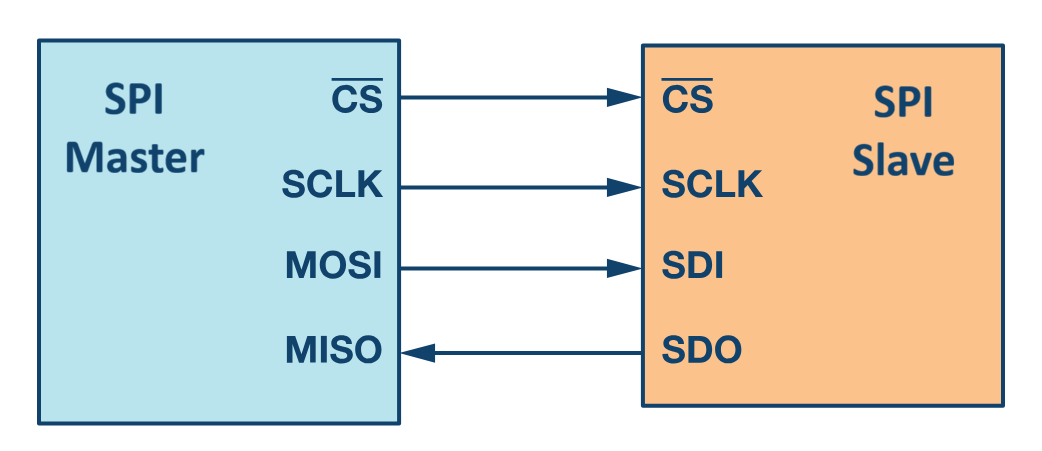
\includegraphics[width = 0.5\textwidth]{media/SPIDiagram.png}
\caption{SPI Configuration of Master and Slave}
\end{figure}

4-wire SPI devices have four signals:
\begin{itemize}
	\item Clock (SPI CLK, SCLK)
    \item Chip select (CS)
    \item Master out, slave in (MOSI)
    \item Master in, slave out (MISO)
\end{itemize}

The device that generates the clock signal is called the master. Data transmitted between the master and the slave is synchronized to the clock generated by the master. SPI devices support much higher clock frequencies compared to I2C interfaces.

The chip select (CS) signal is used by the main device to choose which slave communicates on the SPI bus. It is active low, meaning the slave is selected when the signal is low and disconnected when it is high. If multiple slaves are present, each one needs its own separate chip select line.

MOSI (Master Out Slave In) carries data from the main device to the slave, while MISO (Master In Slave Out) carries data from the slave back to the main device.

\subsection{Data Transmission between the Master and Slave}
To start SPI communication, the master generates the clock signal and selects the slave by pulling the chip select (CS) line low (active low). SPI operates in full-duplex mode, meaning the master and slave can transmit data simultaneously via MOSI and MISO.

During communication, data is shifted out serially while data is also read in at the same time. The clock signal synchronizes this shifting and sampling process. The SPI interface allows flexibility in choosing whether data is sampled or shifted on the rising or falling clock edge. The number of transmitted data bits depends on the specific device. 

\subsection{Clock Polarity and Clock Phase}
In SPI communication, the master configures the clock behavior using two control bits: Clock Polarity (CPOL) and Clock Phase (CPHA). The CPOL bit defines the idle state of the clock signal, i.e., whether the clock remains low (CPOL = 0) or high (CPOL = 1) when no data transmission is taking place. The idle state occurs when the chip select (CS) signal is inactive and at the beginning and end of a transmission.

The CPHA bit determines the clock edge on which data is sampled and shifted. Depending on the configuration, data is captured on either the first or the second clock edge within a clock cycle.

The master must configure CPOL and CPHA according to the timing requirements specified in the slave device’s datasheet. The combination of these two bits results in four possible SPI modes (Mode 0 to Mode 3), each defining a specific clock polarity and phase configuration.

\begin{table}[H]
\begin{tabularx}{\textwidth}{|c|c|c|X|X|}
\hline 
\textbf{SPI Mode} & \textbf{CPOL} & \textbf{CPHA} & \textbf{Clock Polarity in idle state} & \textbf{Clock Phase Used to Sample and/or Shift the Data} \\ \hline 
0 & 0 & 0 & Logic Low & Data sampled on rising edge and shifted out on the falling edge \\ \hline 
1 & 0 & 1 & Logic Low & Data sampled on the falling edge and shifted out on the rising edge \\ \hline
2 & 1 & 0 & Logic High & Data sampled on the falling edge and shifted out on the rising edge \\ \hline
3 & 1 & 1 & Logic High & Data sampled on the rising edge and shifted out on the falling edge \\ \hline
\end{tabularx}
\caption{SPI Modes with CPOL and CPHA}
\end{table}

The following figure illustrate example SPI communication in the four SPI modes, showing data transfer on the MOSI and MISO lines. The start and end of transmission are marked by dotted green lines, while the sampling and shifting edges are indicated in orange and blue, respectively. These figures are provided for illustration only; for reliable SPI communication, the device’s datasheet must be consulted to ensure all timing requirements are satisfied.

\begin{figure}[H]
\centering 
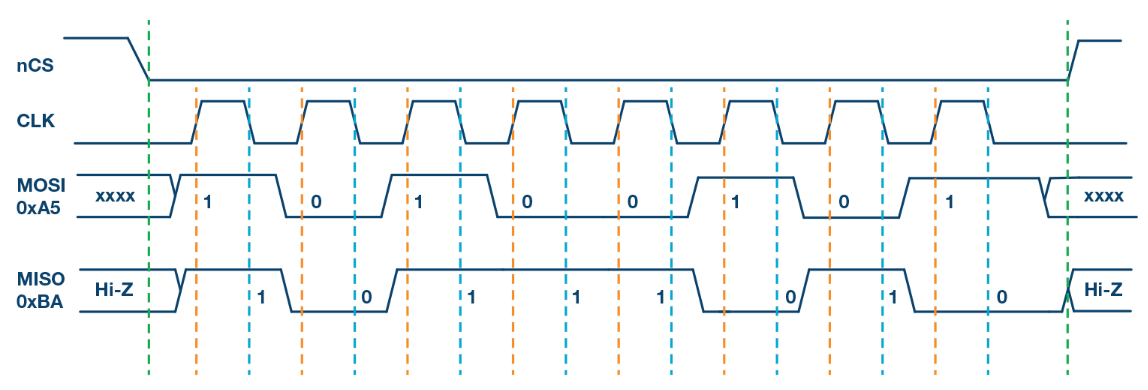
\includegraphics[width = 0.9\textwidth]{media/diagram1.png}
\caption{SPI Mode 0, CPOL = 0, CPHA = 0: CLK idle state = low, data sampled on rising edge and shifted on falling edge}
\label{fig-diagram1}
\end{figure}

 Figure \autoref{fig-diagram2} presents the timing diagram for SPI Mode 1. In this mode, CPOL = 0, meaning the clock remains low during the idle state, and CPHA = 1, meaning data is sampled on the falling clock edge and shifted on the rising clock edge

\begin{figure}[H]
\centering 
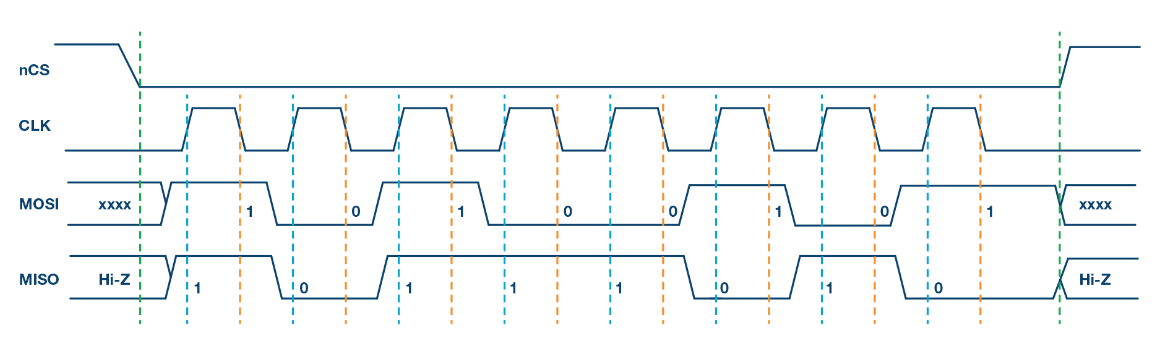
\includegraphics[width = 0.9\textwidth]{media/diagram2.png}
\caption{SPI Mode 1, CPOL = 0, CPHA = 1: CLK idle state = low, data sampled on the falling edge and shifted on the rising edge}
\label{fig-diagram2}
\end{figure}

Figure \ref{fig-diagram3} shows the timing diagram for SPI Mode 2. In this mode, the clock polarity is 1, which indicates that the idle state of the clock signal is high. The clock phase in this mode is 0, which indicates that the data is sampled on the falling edge (shown by the orange dotted line) and the data is shifted on the rising edge (shown by the dotted blue line) of the clock signal.
\begin{figure}[H]
\centering 
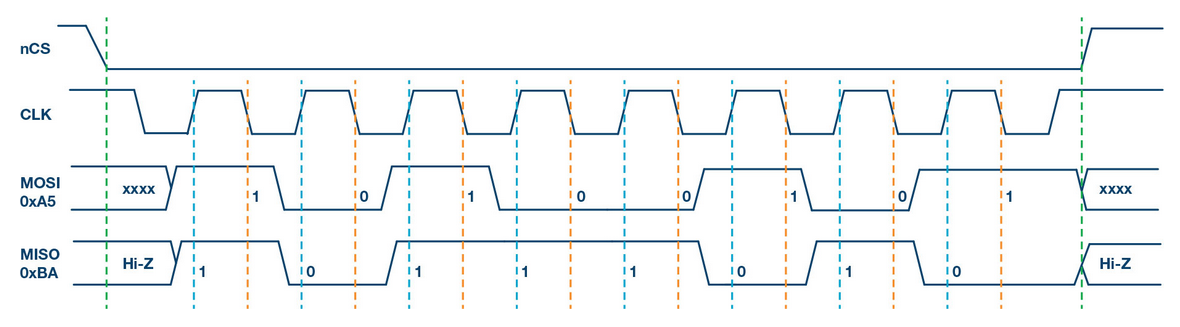
\includegraphics[width = 0.9\textwidth]{media/diagram3.png}
\caption{SPI Mode 2, CPOL = 1, CPHA = 0: CLK idle state = high, data sampled on the falling edge and shifted on the rising edge}
\label{fig-diagram3}
\end{figure}

\autoref{fig-diagram4} shows the timing diagram for SPI Mode 3. In this mode, the clock polarity is 1, which indicates that the idle state of the clock signal is high. The clock phase in this mode is 1, which indicates that the data is sampled on the rising edge (shown by the orange dotted line) and the data is shifted on the falling edge (shown by the dotted blue line) of the clock signal.
\begin{figure}[H]
\centering 
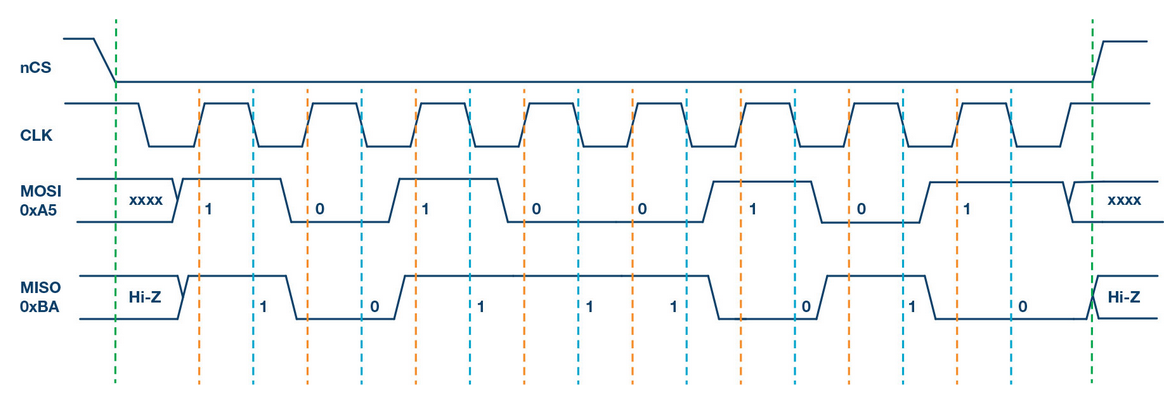
\includegraphics[width = 0.9\textwidth]{media/diagram4.png}
\caption{SPI Mode 3, CPOL = 1, CPHA = 1: CLK idle state = high, data sampled on the rising edge and shifted on the falling edge}
\label{fig-diagram4}
\end{figure}

In SPI systems, a single master can interface with multiple slaves using either a regular or daisy-chain configuration. In the regular mode, each slave requires a dedicated chip select line from the master. When a chip select is pulled low, the corresponding slave is enabled for communication, while enabling multiple slaves simultaneously can corrupt the data on the MISO line. As the number of slaves increases, the number of chip select lines also increases, which may require additional techniques such as multiplexers to manage the connections. In contrast, the daisy-chain configuration connects the slaves in series, allowing data to propagate through each device. This reduces the number of chip select lines needed but increases the number of clock cycles required to reach slaves further down the chain. Each method has trade-offs, and the master must configure the interface according to the specific requirements of the connected slave devices.

\section{SPI in VHDL}
Here in this project we are using an A/D converter, Temperature sensor through the Pmods connectors to the board and the GPIOs present on the Zedboard. \\
for the communication of the A/D converter we need the SPI communication protocol and therefore we need to implment it using VHDL language on the fabric on FPGA. \\
To enable communication between the FPGA and the external A/D converter, the Serial Peripheral Interface (SPI) communication protocol is employed. Since the A/D converter uses SPI as its communication interface, the protocol is implemented directly in VHDL within the programmable logic (FPGA fabric) of the ZedBoard. This approach allows precise timing control and reliable data acquisition without relying on the processing system.\\
The SPI communication protocol is a synchronous serial interface commonly used for short-distance communication between a master device and one or more slave peripherals. In the implemented system, the FPGA operates as the SPI master, while the A/D converter functions as the SPI slave. Communication is initiated and controlled entirely by the master, which generates the clock signal and manages the data transfer sequence.\\
SPI communication is based on four primary signals: Serial Clock (SCLK), Master Out Slave In (MOSI), Master In Slave Out (MISO), and Chip Select (CS). The SCLK signal is generated by the FPGA and defines the timing of data transmission. The MOSI line is used to send control or configuration data from the FPGA to the A/D converter, while the MISO line is used to receive the digitized output data from the converter. The CS signal is used to select and activate the A/D converter during communication, ensuring that data exchange occurs only when intended.\\
The SPI master is implemented in VHDL as a dedicated hardware module. This module generates the required clock signal, controls the chip select line, and manages the serial shifting of data in accordance with the timing requirements specified in the A/D converter datasheet. Data is transmitted and sampled synchronously with the SPI clock, following the defined clock polarity and phase configuration.

A finite state machine (FSM) is used to control the SPI communication process. The FSM manages the different stages of operation, including the idle state, activation of the chip select signal, serial data transmission, data reception, and termination of communication. This structured control mechanism ensures deterministic behavior and reliable data transfer, which are essential for accurate temperature measurement.

Implementing the SPI protocol in FPGA hardware offers several advantages, such as deterministic timing, low latency, and independence from software execution delays. This makes the design well suited for real-time and embedded applications, where consistent and reliable communication with external sensors and converters is required. Additionally, the VHDL-based implementation allows flexibility in adjusting parameters such as clock frequency and data length to support different SPI-compatible devices. \cite{mohammadi-spi-vhdl}

\subsection{SPI master \texttt{CPOL = 0, CPHA = 1}}
The following examples shows the implementation of SPI communication protocol for a master with \texttt{CPO = 0, CPHA = 1}, the example shows the data communication for an 8 bit SPI communication. 
The SPI implementation uses a Finit State Machine that controls the data flow, synchronization logic for SPI clock generation and shift registers for data handling. 

\subsection{Description of the SPI using FSM (Finite State Machine)}
The design implements an SPI (Serial Peripheral Interface) transmitter module configured for mode \texttt{(CPOL = 0, CPHA = 1)} with 8-bit data communication. The design includes a finite state machine (FSM) that manages the different stages of SPI communication: idle, start, data transmission (clock high and low phases), and stop. It uses internal shift registers to handle serial transmission (sdo) and reception (sdi) of data bits. A clock divider is implemented to generate a slower SPI clock \texttt{(spi\_clkp)} derived from the input clock (bclk). The scsq signal acts as the
chip select, active low, and sclk is the SPI clock output. 

\begin{figure}[H]
\centering 
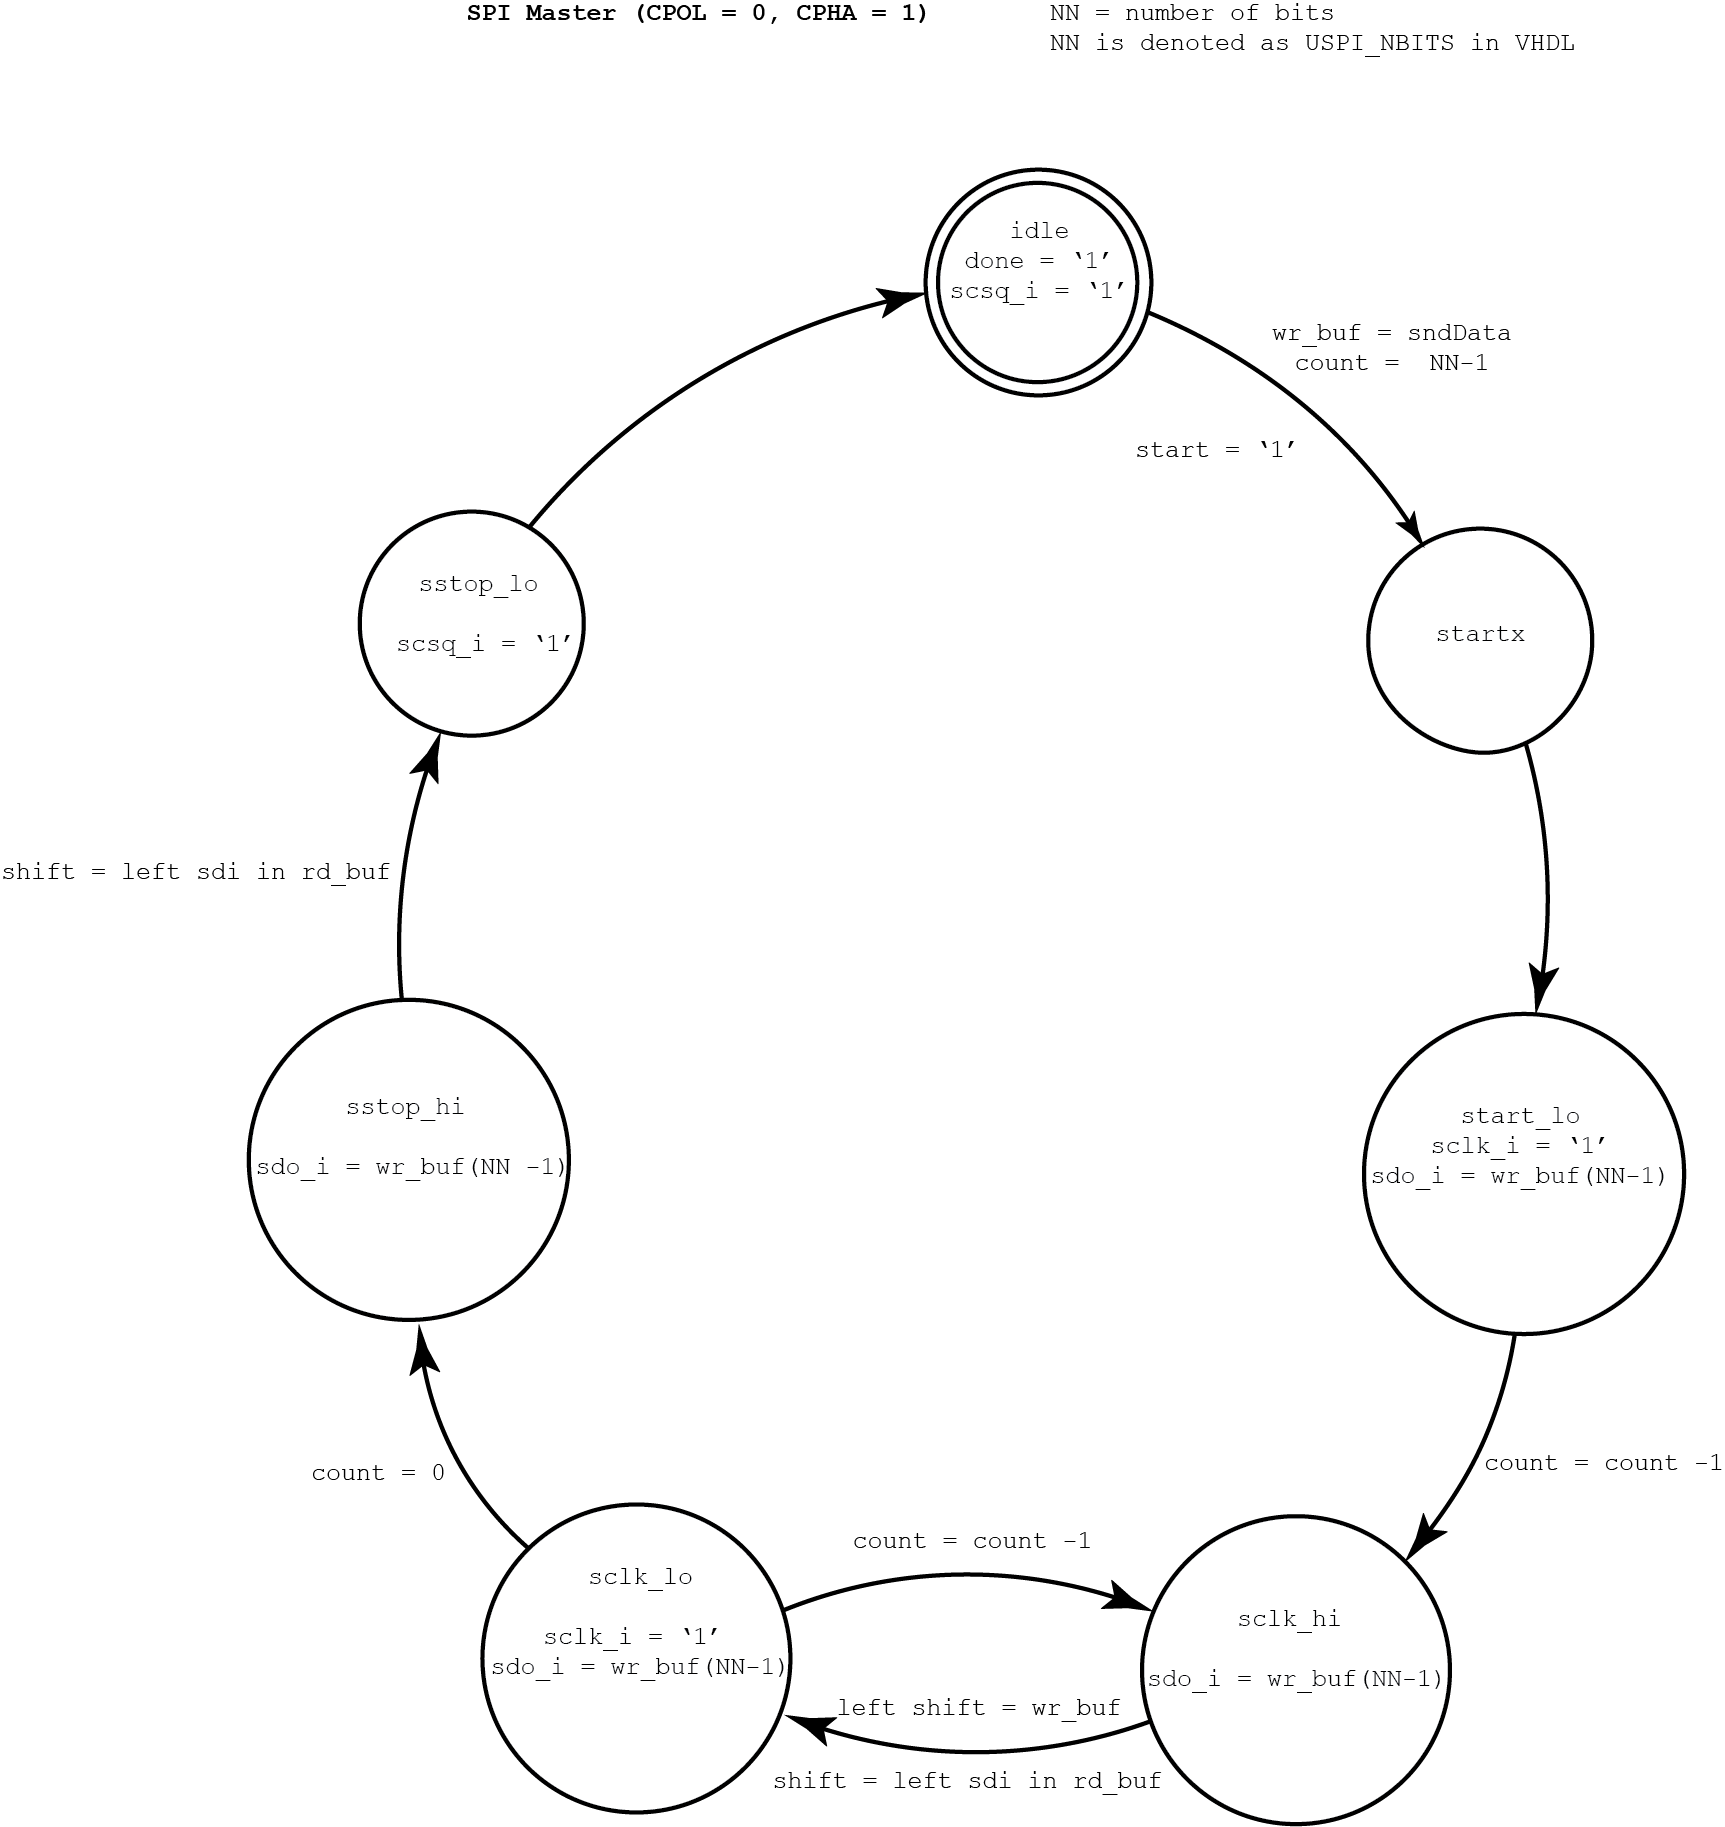
\includegraphics[width = 0.95\textwidth]{media/spi_master.png}
\caption{SPI Master State Machine Diagram}
\label{fig-state_machine}
\end{figure}
The following VHDL codes shows the implementation of the above SPI Master: 
\begin{minted}[bgcolor = lightgray, tabsize = 4, breaklines, numbers = left]{vhdl}
------------------------------------------------------------------------
-- Engineer: Mohammad Mahdi Mohammadi
-- Module Name: spicpol0cph1 - Behavioral
-- Description: SPI transmitter cpol=0, cphase = 1, 8bit.
------------------------------------------------------------------------
LIBRARY IEEE;
USE IEEE.STD_LOGIC_1164.ALL;
ENTITY spicpol0chp1 IS
    PORT (
        reset : IN STD_LOGIC;
        bclk : IN STD_LOGIC;
        start : IN STD_LOGIC;
        done : OUT STD_LOGIC;
        scsq : OUT STD_LOGIC;
        sclk : OUT STD_LOGIC;
        sdi : IN STD_LOGIC;
        sdo : OUT STD_LOGIC;
        sndData : IN STD_LOGIC_VECTOR (7 DOWNTO 0);
        rcvData : OUT STD_LOGIC_VECTOR (7 DOWNTO 0));
END spicpol0chp1;

ARCHITECTURE Behavioral OF spicpol0chp1 IS
    CONSTANT SPI_NBITS : INTEGER := 8;
    TYPE STATE_TYPE IS (sidle, sstartx, sstart_lo, sclk_hi, sclk_lo, sstop_hi, sstop_lo);
    SIGNAL state, next_state : state_type;
    SIGNAL scsq_i, sclk_i, sdo_i : STD_LOGIC;
    SIGNAL lshift : STD_LOGIC;
    SIGNAL start_i : STD_LOGIC;
    SIGNAL wr_buf : STD_LOGIC_VECTOR (SPI_NBITS - 1 DOWNTO 0);
    SIGNAL rd_buf : STD_LOGIC_VECTOR (SPI_NBITS - 1 DOWNTO 0);
    SIGNAL count : INTEGER RANGE 0 TO SPI_NBITS - 1;
    -- for simulation
    CONSTANT clk_div : INTEGER := 3;
    -- for hardware test 5 bits / sec transmission rate
    --constant CLK_DIV : integer := 9999999;
    SUBTYPE counter_type IS INTEGER RANGE 0 TO clk_div;
    SIGNAL SPI_CLKP : STD_LOGIC;
BEGIN
    CLKDIV_P : PROCESS (BCLK)
        VARIABLE cnt : counter_type := clk_div;
    BEGIN
        IF rising_edge (bclk) THEN
            spi_clkp <= '0';
            IF cnt = 0 THEN
                spi_clkp <= '1';
                cnt := clk_div;
            ELSE
                cnt := cnt - 1;
            END IF;
        END IF;
        Complete Source code OF SPI
        8
    END PROCESS clkdiv_p;
    rcvData <= rd_buf;
    seq_p : PROCESS (bclk)
    BEGIN
        IF rising_edge(bclk) THEN
            start_i <= start;
            -- if spi_clkp = '1' then
            IF reset = '1' THEN
                state <= sidle;
                -- scsq <= '0';
                sclk <= '0';
                sdo <= '0';
            ELSE
                IF next_state = sstartx THEN
                    count <= SPI_NBITS - 1;
                    wr_buf <= sndData;
                ELSIF next_state = sclk_hi THEN
                    count <= count - 1;
                ELSIF next_state = sclk_lo THEN
                    wr_buf <= wr_buf(SPI_NBITS - 2 DOWNTO 0) & '-';
                    rd_buf <= rd_buf(SPI_NBITS - 2 DOWNTO 0) & sdi;
                ELSIF next_state = sstop_lo THEN
                    rd_buf <= rd_buf(SPI_NBITS - 2 DOWNTO 0) & sdi;
                END IF;
                state <= next_state;
                scsq <= scsq_i;
                sclk <= sclk_i;
                sdo <= sdo_i;
                -- end if;
            END IF;
        END IF;
    END PROCESS seq_p;

    cmb_p : PROCESS (state, start_i, count, wr_buf)
    BEGIN
        next_state <= state;
        scsq_i <= '0';
        sclk_i <= '0';
        sdo_i <= '0';
        done <= '0';
        CASE state IS
            WHEN sidle =>
                done <= '1';
                scsq_i <= '1';
                IF start_i = '1' THEN
                    next_state <= sstartx;
                END IF;
            WHEN sstartx =>
                next_state <= sstart_lo;
            WHEN sstart_lo =>
                sclk_i <= '1';
                sdo_i <= wr_buf(SPI_NBITS - 1);
                next_state <= sclk_hi;
            WHEN sclk_hi =>
                sdo_i <= wr_buf(SPI_NBITS - 1);
                next_state <= sclk_lo;
            WHEN sclk_lo =>
                sclk_i <= '1';
                sdo_i <= wr_buf(SPI_NBITS - 1);
                IF count = 0 THEN
                    next_state <= sstop_hi;
                ELSE
                    next_state <= sclk_hi;
                END IF;
            WHEN sstop_hi =>
                Top Level FILE
                9
                sdo_i <= wr_buf(SPI_NBITS - 1);
                next_state <= sstop_lo;
            WHEN sstop_lo =>
                scsq_i <= '1';
                next_state <= sidle;
        END CASE;
    END PROCESS cmb_p;
END Behavioral;
\end{minted}

\section{Section 2: Hardware Design of Measurement Network Gateway}
	One of the most important part of this project is the use of Embedded Linux in zynq7000 FPGA on ZedBoard Evaluation Board. The hardware required for this project is developed inside Vivado in VHDL language.\\
	The system shall acquire data from a precision resistive temperature sensor, two ADCs, onboard Switches and Push Buttons. \\
	For this reason a new custom AXI slave IP has been created inside Vivado and this Ip has the following hierarchy structure.
	\begin{figure}[H]
	\begin{center}
	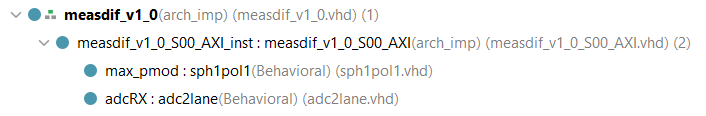
\includegraphics[width = 0.75\textwidth]{media/hstructure.png}
	\caption{Hierarchy Structure of the Custom AXI slave IP in Vivado}
	\end{center}
	\end{figure} 
	\subsection{Description of the file: adc2lane.vhd}
	This file is made to acquire data from two ADCs based on SPI (CPOL=0, CPHA=1) communication protocal. \\
	The entity adc2lane is a configurable SPI receiver that operates with two input data channels (sdi\_0 and sdi\_1) in parallel, capturing data words of configurable length (USPI\_SIZE, default 16 bits). It communicates synchronously using SPI mode settings CPOL=0 and CPHA=1.
	The following is the VHDL code for the implemenation of acquiring data from the ADCs using SPI. 
	
	\textbf{Inputs:}
	\begin{enumerate}
	\item resetn: Active-low synchronous reset.
	\item bclk: Base clock for FSM timing.
	\item spi\_clkp: SPI clock polarity indicator (CPOL=0 here).
	\item start: Signal to begin data acquisition.
	\item sdi\_0, sdi\_1: Serial data inputs from two ADC lanes.
	\end{enumerate}
	\textbf{Outputs:}
	\begin{enumerate}
	\item done: Signal asserted when data reception is complete.
	\item scsq: SPI chip select line, active low.
	\item sclk: SPI clock output.
	\item rcvData\_0, rcvData\_1: Received data vectors from both SPI lanes.
	\end{enumerate}
	At the beginning of the VHDL program, the standard libraries are used: 
\begin{minted}[breaklines, tabsize = 4, bgcolor = lightgray]{VHDL}
library IEEE;
use IEEE.STD_LOGIC_1164.ALL;
\end{minted}

are included to make standard logic types and definitions available for the design. The library IEEE; statement declares the use of the IEEE library, which contains commonly used packages, while use \texttt{IEEE.STD\_LOGIC\_1164.ALL;} imports all definitions from the \texttt{STD\_LOGIC\_1164} package.
	
This package provides the std\_logic and std\_logic\_vector types, which support multiple logic values (such as 0, 1, Z, and X) and are essential for modeling digital signals and buses. Including these lines ensures that the designer can use standard logic data types and operations throughout the VHDL code.\\

After adding the standard libraries, the input and output of the IP is defined as follows:
\begin{minted}[breaklines, tabsize = 4, bgcolor = lightgray]{VHDL}
entity adc2lane is
    GENERIC ( USPI_SIZE : INTEGER := 16 );
    Port ( resetn : in STD_LOGIC;
       bclk : in STD_LOGIC;
       spi_clkp : in STD_LOGIC;
       start : in STD_LOGIC;
       done : out STD_LOGIC;
       scsq : out STD_LOGIC;
       sclk : out STD_LOGIC;
       sdi_0 : in STD_LOGIC;
       sdi_1 : in STD_LOGIC;
       rcvData_0 : out STD_LOGIC_VECTOR (USPI_SIZE-1 downto 0);
       rcvData_1 : out STD_LOGIC_VECTOR (USPI_SIZE-1 downto 0));
end adc2lane;
\end{minted}
 
In this VHDL design, custom enumerated types are defined to represent the states of two finite state machines (FSMs). The type \texttt{state\_type} defines six states (\texttt{sidle}, \texttt{sstartx}, \texttt{sclk\_lo}, \texttt{sclk\_hi}, \texttt{sstop\_lo}, \texttt{sstop\_hi}) for controlling the SPI clock and data transmission, with corresponding signals \texttt{state} and \texttt{next\_state} used to hold the current and next states. The SPI signals \texttt{sclk\_i} and \texttt{scsq\_i} are declared as \texttt{STD\_LOGIC}, while two read buffers, \texttt{rd\_buf\_0} and \texttt{rd\_buf\_1}, are defined as \texttt{STD\_LOGIC\_VECTOR} arrays of size \texttt{USPI\_SIZE}. A counter signal \texttt{count} is used to track the bit position during SPI transfers. Additionally, a second FSM for slave select control is defined using the type \texttt{sslst\_type} with three states (\texttt{ssl\_idle}, \texttt{ssl\_start}, \texttt{ssl\_run}), with \texttt{ssl\_state} and \texttt{sslnxt\_state} representing the current and next states. The signal \texttt{start\_i} acts as an input trigger for initiating the slave select sequence. This structured use of enumerated types and signals ensures clear and organized control over the SPI communication process.

\begin{minted}[breaklines, tabsize = 4, bgcolor = lightgray]{VHDL}
architecture Behavioral of adc2lane is

type state_type IS (sidle, sstartx, sclk_lo, sclk_hi, sstop_lo, sstop_hi);
SIGNAL  state, next_state: state_type;
SIGNAL sclk_i, scsq_i : STD_LOGIC;
SIGNAL rd_buf_0, rd_buf_1 : STD_LOGIC_VECTOR(USPI_SIZE-1 downto 0);
SIGNAL count : integer RANGE 0 TO USPI_SIZE-1;

type sslst_type IS (ssl_idle, ssl_start, ssl_run);
SIGNAL ssl_state, sslnxt_state: sslst_type;
SIGNAL start_i : STD_LOGIC;
\end{minted}

The following assignment:
\begin{minted}[breaklines, tabsize = 4, bgcolor = lightgray]{VHDL}
begin

    rcvData_0 <= rd_buf_0;
    rcvData_1 <= rd_buf_1;
\end{minted}

are used to transfer the contents of the internal read buffers to the output signals. Here, \texttt{rd\_buf\_0} and \texttt{rd\_buf\_1} hold the data received from the SPI interface, and by assigning them to \texttt{rcvData\_0} and \texttt{rcvData\_1}, the received data is made available for use in other parts of the design or for further processing. This ensures that the SPI data captured in the buffers is properly output from the module while maintaining synchronization with the system clock.


\begin{minted}[breaklines, tabsize = 4, bgcolor = lightgray]{VHDL}
	-- start/stop logic
	-- proper handling of clock division
	sslseq_proc: PROCESS(resetn, bclk, sslnxt_state)
	BEGIN
		IF rising_edge(bclk) THEN
			IF resetn='0' THEN
				ssl_state <= ssl_idle;
			ELSE
				ssl_state <= sslnxt_state;
			END IF;
		END IF;
	END PROCESS sslseq_proc;
\end{minted}

The \texttt{sslseq\_proc} process implements a finite state machine (FSM) to control the SPI slave select (SS) signal. It updates the current state (\texttt{ssl\_state}) synchronously on the rising edge of the base clock (\texttt{bclk}) and can be reset to the idle state (\texttt{ssl\_idle}) when \texttt{resetn} is low, ensuring the slave is properly deselected on system reset. By sequencing through defined states such as idle, start, and run, the process determines when the slave is selected and for how long, effectively controlling the timing of the SS signal. The FSM can remain in a particular state for multiple clock cycles, which produces a clock division effect that guarantees the slave is enabled for the correct duration during SPI data transfers. This structure ensures precise, clock-synchronized selection and deselection of the slave device, providing reliable SPI communication without requiring additional timing hardware.



\begin{minted}[breaklines, tabsize = 4, bgcolor = lightgray]{VHDL}
	sslcmb_proc: PROCESS(ssl_state, state, start)
	BEGIN
		sslnxt_state <= ssl_state;
		start_i <= '0';
		done <= '0';
		CASE ssl_state IS
			WHEN ssl_idle =>
				done <= '1';
				IF start='1' AND state=sidle THEN
					sslnxt_state <= ssl_start;
				END IF;
			WHEN ssl_start =>
				start_i <= '1';
				IF state=sstartx THEN
					sslnxt_state <= ssl_run;
				END IF;
			WHEN ssl_run =>
				IF state=sidle THEN
					sslnxt_state <= ssl_idle;
				END IF;
		END CASE;
	END PROCESS sslcmb_proc;
\end{minted}

The \texttt{sslcmb\_proc} process implements the combinational logic for the slave select finite state machine (FSM) in the SPI interface. It determines the next state (\texttt{sslnxt\_state}) and controls the output signals \texttt{start\_i} and \texttt{done} based on the current FSM state (\texttt{ssl\_state}), the SPI transmission state (\texttt{state}), and the \texttt{start} input signal. In the idle state (\texttt{ssl\_idle}), \texttt{done} is set to \textquotesingle 1\textquotesingle{} to indicate that the SPI transmission is finished, and if \texttt{start} = \textquotesingle 1\textquotesingle{} while the SPI FSM is idle (\texttt{sidle}), the FSM transitions to \texttt{ssl\_start}. In the \texttt{ssl\_start} state, \texttt{start\_i} is set to \textquotesingle 1\textquotesingle{} to initiate the slave select activation, and once the SPI FSM reaches the \texttt{sstartx} state, the FSM moves to \texttt{ssl\_run}. During \texttt{ssl\_run}, the slave select signal remains active while data is being transferred, and the FSM returns to \texttt{ssl\_idle} once the SPI FSM returns to \texttt{sidle}. This process ensures proper timing and sequencing of the slave select signal, coordinating its activation and deactivation with the SPI transmission without requiring additional sequential logic.



\begin{minted}[breaklines, tabsize = 4, bgcolor = lightgray]{VHDL}
	-- spi logic
	sseq_proc: PROCESS(resetn, bclk, next_state, sclk_i, scsq_i,
				       rd_buf_0, rd_buf_0, sdi_0, sdi_1, count, spi_clkp)
	BEGIN
		IF rising_edge(bclk) THEN
			IF resetn='0' THEN
				state <= sidle;
				count <= USPI_SIZE-1;
			ELSIF spi_clkp='1' THEN
				IF next_state=sstartx THEN
                count <= USPI_SIZE - 1;
                ELSIF next_state=sclk_lo THEN
                    count <= count - 1;
                    rd_buf_0 <= rd_buf_0(USPI_SIZE-2 downto 0) & sdi_0;
                    rd_buf_1 <= rd_buf_1(USPI_SIZE-2 downto 0) & sdi_1;
                ELSIF next_state=sstop_lo THEN
                    rd_buf_0 <= rd_buf_0(USPI_SIZE-2 downto 0) & sdi_0;
                    rd_buf_1 <= rd_buf_1(USPI_SIZE-2 downto 0) & sdi_1;
                END IF;
                state <= next_state;
                sclk <= sclk_i;
                scsq <= scsq_i;
			END IF;
		END IF;
	END PROCESS sseq_proc;
\end{minted}

The \texttt{sseq\_proc} process implements the main SPI logic, managing both the data reception and the finite state machine (FSM) that controls the SPI interface. It operates synchronously on the rising edge of the base clock (\texttt{bclk}) and responds to the reset signal (\texttt{resetn}) and the SPI clock enable signal (\texttt{spi\_clkp}). When the reset is active (\texttt{resetn = '0'}), the FSM state is initialized to \texttt{sidle} and the bit counter is set to \texttt{USPI\_SIZE-1}, ensuring that the SPI interface starts in a known idle state.

During normal operation, the process monitors the FSM states to control data reception and state transitions. In the \texttt{sstartx} state, the bit counter is reset to prepare for receiving a new SPI word. In the \texttt{sclk\_lo} state, the counter decrements for each clock cycle, and the incoming serial data bits (\texttt{sdi\_0} and \texttt{sdi\_1}) are shifted into the read buffers (\texttt{rd\_buf\_0} and \texttt{rd\_buf\_1}), performing serial-to-parallel conversion. In the \texttt{sstop\_lo} state, the final bits of the SPI word are shifted into the buffers to complete the data reception.

At each enabled clock cycle, the FSM updates the current state to the next state (\texttt{next\_state}), while the SPI clock (\texttt{sclk}) and slave select clock (\texttt{scsq}) signals are updated from their internal signals (\texttt{sclk\_i} and \texttt{scsq\_i}). This process ensures proper timing and sequencing of the SPI FSM, accurate serial-to-parallel conversion of received data, and synchronized control of the SPI clock and slave select signals, enabling reliable SPI communication.


\begin{minted}[breaklines, tabsize = 4, bgcolor = lightgray]{VHDL}
	scmb_proc: PROCESS(state, start_i, count)
	BEGIN
		next_state <= state;
		sclk_i <= '1';
		scsq_i <= '0';
		CASE state IS
			WHEN sidle =>
				scsq_i <= '1';
				IF start_i='1' THEN
					next_state <= sstartx;
				END IF;
			WHEN sstartx =>
                next_state <= sclk_hi;
			WHEN sclk_hi =>
                sclk_i <= '0';
                IF count=0 THEN
                    next_state <= sstop_lo;
                ELSE
                    next_state <= sclk_lo;
                END IF;
            WHEN sclk_lo =>
				next_state <= sclk_hi;
			WHEN sstop_lo =>
				next_state <= sstop_hi;
			WHEN sstop_hi =>
				scsq_i <= '1';
				next_state <= sidle;
		END CASE;
	END PROCESS scmb_proc;

end Behavioral;
\end{minted}

The \texttt{scmb\_proc} process implements the combinational logic for controlling the SPI clock (\texttt{sclk\_i}) and slave select (\texttt{scsq\_i}) signals based on the current FSM state (\texttt{state}), the start signal (\texttt{start\_i}), and the bit counter (\texttt{count}). In the idle state (\texttt{sidle}), the slave select is high, and if \texttt{start\_i} is active, the FSM moves to \texttt{sstartx} to begin a transaction. The FSM then alternates between \texttt{sclk\_hi} and \texttt{sclk\_lo} to generate clock pulses, using the bit counter to determine when the data transfer is complete. After the last bit, the FSM transitions through \texttt{sstop\_lo} and \texttt{sstop\_hi}, sets the slave select high, and returns to \texttt{sidle}, completing the SPI transaction. This process ensures correct clock generation, slave selection, and sequencing for reliable SPI communication.\\

Here is the complete VHDL code for this program. 
\begin{minted}[breaklines, tabsize = 4, bgcolor = lightgray, numbers=left]{VHDL}
----------------------------------------------------------------------------------
-- Company:         Univ. Bremerhaven
-- Engineer:        Kai Mueller
-- 
-- Create Date:     08.06.2016 00:15:32
-- Description:     ADC 2 Lanes SPI based on spipol1pha0 template (CPOL=0 CPHA=1)
-- 
----------------------------------------------------------------------------------

library IEEE;
use IEEE.STD_LOGIC_1164.ALL;

entity adc2lane is
    GENERIC ( USPI_SIZE : INTEGER := 16 );
    Port ( resetn : in STD_LOGIC;
       bclk : in STD_LOGIC;
       spi_clkp : in STD_LOGIC;
       start : in STD_LOGIC;
       done : out STD_LOGIC;
       scsq : out STD_LOGIC;
       sclk : out STD_LOGIC;
       sdi_0 : in STD_LOGIC;
       sdi_1 : in STD_LOGIC;
       rcvData_0 : out STD_LOGIC_VECTOR (USPI_SIZE-1 downto 0);
       rcvData_1 : out STD_LOGIC_VECTOR (USPI_SIZE-1 downto 0));
end adc2lane;

architecture Behavioral of adc2lane is

type state_type IS (sidle, sstartx, sclk_lo, sclk_hi, sstop_lo, sstop_hi);
SIGNAL  state, next_state: state_type;
SIGNAL sclk_i, scsq_i : STD_LOGIC;
SIGNAL rd_buf_0, rd_buf_1 : STD_LOGIC_VECTOR(USPI_SIZE-1 downto 0);
SIGNAL count : integer RANGE 0 TO USPI_SIZE-1;

type sslst_type IS (ssl_idle, ssl_start, ssl_run);
SIGNAL ssl_state, sslnxt_state: sslst_type;
SIGNAL start_i : STD_LOGIC;

begin

    rcvData_0 <= rd_buf_0;
    rcvData_1 <= rd_buf_1;

	-- start/stop logic
	-- proper handling of clock division
	sslseq_proc: PROCESS(resetn, bclk, sslnxt_state)
	BEGIN
		IF rising_edge(bclk) THEN
			IF resetn='0' THEN
				ssl_state <= ssl_idle;
			ELSE
				ssl_state <= sslnxt_state;
			END IF;
		END IF;
	END PROCESS sslseq_proc;

	sslcmb_proc: PROCESS(ssl_state, state, start)
	BEGIN
		sslnxt_state <= ssl_state;
		start_i <= '0';
		done <= '0';
		CASE ssl_state IS
			WHEN ssl_idle =>
				done <= '1';
				IF start='1' AND state=sidle THEN
					sslnxt_state <= ssl_start;
				END IF;
			WHEN ssl_start =>
				start_i <= '1';
				IF state=sstartx THEN
					sslnxt_state <= ssl_run;
				END IF;
			WHEN ssl_run =>
				IF state=sidle THEN
					sslnxt_state <= ssl_idle;
				END IF;
		END CASE;
	END PROCESS sslcmb_proc;

	-- spi logic
	sseq_proc: PROCESS(resetn, bclk, next_state, sclk_i, scsq_i,
				       rd_buf_0, rd_buf_0, sdi_0, sdi_1, count, spi_clkp)
	BEGIN
		IF rising_edge(bclk) THEN
			IF resetn='0' THEN
				state <= sidle;
				count <= USPI_SIZE-1;
			ELSIF spi_clkp='1' THEN
				IF next_state=sstartx THEN
                count <= USPI_SIZE - 1;
                ELSIF next_state=sclk_lo THEN
                    count <= count - 1;
                    rd_buf_0 <= rd_buf_0(USPI_SIZE-2 downto 0) & sdi_0;
                    rd_buf_1 <= rd_buf_1(USPI_SIZE-2 downto 0) & sdi_1;
                ELSIF next_state=sstop_lo THEN
                    rd_buf_0 <= rd_buf_0(USPI_SIZE-2 downto 0) & sdi_0;
                    rd_buf_1 <= rd_buf_1(USPI_SIZE-2 downto 0) & sdi_1;
                END IF;
                state <= next_state;
                sclk <= sclk_i;
                scsq <= scsq_i;
			END IF;
		END IF;
	END PROCESS sseq_proc;

	scmb_proc: PROCESS(state, start_i, count)
	BEGIN
		next_state <= state;
		sclk_i <= '1';
		scsq_i <= '0';
		CASE state IS
			WHEN sidle =>
				scsq_i <= '1';
				IF start_i='1' THEN
					next_state <= sstartx;
				END IF;
			WHEN sstartx =>
                next_state <= sclk_hi;
			WHEN sclk_hi =>
                sclk_i <= '0';
                IF count=0 THEN
                    next_state <= sstop_lo;
                ELSE
                    next_state <= sclk_lo;
                END IF;
            WHEN sclk_lo =>
				next_state <= sclk_hi;
			WHEN sstop_lo =>
				next_state <= sstop_hi;
			WHEN sstop_hi =>
				scsq_i <= '1';
				next_state <= sidle;
		END CASE;
	END PROCESS scmb_proc;

end Behavioral;
\end{minted}

\subsection{Description of the file: sph1pol1.vhd}
The VHDL module implements an SPI master used to interface with the MAX31865 Pmod. The MAX31865 converts the resistance of an RTD sensor into a digital value accessible via SPI. Communication is initiated by asserting the start signal, which triggers the internal FSM to activate the chip select (scsq) and begin serial data transfer.

Input data (sndData) containing register addresses or commands is loaded into an internal shift register (wr\_buf) and transmitted bit by bit on sdo, while incoming bits from sdi are captured in rd\_buf. A counter ensures all USPI\_SIZE bits are transferred. After the transaction, scsq is deactivated and the received data is available on rcvData, representing the RTD measurement.

The SPI clock (sclk) idle state corresponds to CPOL = 1, and data shifting and sampling occur in alternating clock phases as defined by the FSM. This design provides a reliable, FSM-based SPI master capable of configuring and reading the MAX31865 Pmod.\\
It exposes the following ports:\\
\textbf{Inputs:}
\begin{enumerate}
\item resetn: Active-low reset signal for synchronous initialization.
\item bclk: Base clock signal used to drive internal FSM timing.
\item spi\_clkp: Indicates the SPI clock polarity (CPOL=1 in this design).
\item start: Initiates an SPI transaction.
\item sdi: Serial data input from the slave device.
\item sndData: Data vector to be transmitted through MOSI.
\end{enumerate}
\textbf{outputs:}
\begin{enumerate}
\item done: Signal asserted at the completion of an SPI transaction.
\item scsq: Chip select output, active low for SPI device enabling.
\item sclk: SPI clock output.
\item sdo: Serial data output to the slave device.
\item rcvData: Received data vector collected from MISO.
\end{enumerate}

\begin{minted}[breaklines, tabsize = 4, bgcolor = lightgray]{VHDL}
library IEEE;
use IEEE.STD_LOGIC_1164.ALL;

entity sph1pol1 is
    GENERIC ( USPI_SIZE : INTEGER := 16 );
    Port ( resetn : in STD_LOGIC;
            bclk : in STD_LOGIC;
            spi_clkp : in STD_LOGIC;
            start : in STD_LOGIC;
            done : out STD_LOGIC;
            scsq : out STD_LOGIC;
            sclk : out STD_LOGIC;
            sdo : out STD_LOGIC;
            sdi : in STD_LOGIC;
            sndData : in STD_LOGIC_VECTOR (USPI_SIZE-1 downto 0);
            rcvData : out STD_LOGIC_VECTOR (USPI_SIZE-1 downto 0));
end sph1pol1;
\end{minted}

The standard IEEE library is included in this module, and the package \texttt{STD\_LOGIC\_1164.ALL} is imported to provide the required data types such as \texttt{STD\_LOGIC} and \texttt{STD\_LOGIC\_VECTOR}, which are essential for modeling digital signals and multi-bit buses in VHDL.

After including the necessary libraries, the entity \texttt{sph1pol1} is declared to define the external interface of the module. A generic parameter \texttt{USPI\_SIZE : INTEGER := 16} is introduced to configure the SPI data width, allowing flexible word lengths during instantiation.
 
The input ports include \texttt{resetn} as an active-low reset signal, \texttt{bclk} as the base clock, \texttt{spi\_clkp} for SPI clock polarity control, \texttt{start} to initiate transmission, \texttt{sdi} as the serial data input (MISO), and \texttt{sndData} as the parallel data to be transmitted. The output ports include \texttt{done} to indicate completion of transmission, \texttt{scsq} as the chip select signal, \texttt{sclk} as the SPI clock output, \texttt{sdo} as the serial data output (MOSI), and \texttt{rcvData} as the parallel received data. Altogether, this entity defines a configurable SPI master interface capable of transmitting and receiving data words of adjustable length using a simple start--done handshake mechanism.


\begin{minted}[breaklines, tabsize = 4, bgcolor = lightgray]{VHDL}
architecture Behavioral of sph1pol1 is

type state_type IS (sidle, sstartx, sstart_lo, sclk_lo, sclk_hi, stop_hi, stop_lo);
SIGNAL  state, next_state: state_type;
SIGNAL sclk_i, scsq_i, sdo_i : STD_LOGIC;
SIGNAL wr_buf : STD_LOGIC_VECTOR(USPI_SIZE-1 downto 0);
SIGNAL rd_buf : STD_LOGIC_VECTOR(USPI_SIZE-1 downto 0);
SIGNAL count : integer RANGE 0 TO USPI_SIZE-1;

type sslst_type IS (ssl_idle, ssl_start, ssl_run);
SIGNAL ssl_state, sslnxt_state: sslst_type;
SIGNAL start_i : STD_LOGIC;
\end{minted}
In this part of the design, the internal signals and state machines required for SPI communication with the MAX31865 are defined. The first finite state machine (FSM), represented by \texttt{state\_type}, handles the bit-level SPI operations. It controls the chip select, generates the SPI clock, shifts out commands or data through \texttt{sdo\_i}, and reads incoming bits from \texttt{sdi} into the receive buffer \texttt{rd\_buf}. The signal \texttt{count} keeps track of how many bits have been transmitted or received, ensuring that a full \texttt{USPI\_SIZE}-bit word is transferred. The transmit buffer \texttt{wr\_buf} holds the command or configuration data sent to the MAX31865, while \texttt{rd\_buf} stores the sensor's response, including the RTD measurement.

The second FSM, represented by \texttt{sslst\_type}, manages the overall transaction flow. It synchronizes the \texttt{start} signal and ensures that SPI transfers only begin when requested, asserting the \texttt{done} signal when the transaction completes. Together, these FSMs and signals allow the SPI master to reliably configure the MAX31865 and read temperature measurements from the RTD sensor.

\begin{minted}[breaklines, tabsize = 4, bgcolor = lightgray]{VHDL}
begin

	rcvData <= rd_buf;

	-- start/stop logic
	-- proper handling of clock division
	sslseq_proc: PROCESS(resetn, bclk, sslnxt_state)
	BEGIN
		IF rising_edge(bclk) THEN
			IF resetn='0' THEN
				ssl_state <= ssl_idle;
			ELSE
				ssl_state <= sslnxt_state;
			END IF;
		END IF;
	END PROCESS sslseq_proc;
\end{minted}
This part of the code assigns the internal receive buffer \texttt{rd\_buf} to \texttt{rcvData} and updates the start/stop FSM (\texttt{ssl\_state}). On each rising edge of \texttt{bclk}, the FSM resets to \texttt{ssl\_idle} if \texttt{resetn} is low; otherwise, it transitions to the next state (\texttt{sslnxt\_state}), ensuring that SPI transactions remain synchronized with the system clock.

\begin{minted}[bgcolor=lightgray, tabsize=4, breaklines]{vhdl}
	sslcmb_proc: PROCESS(ssl_state, state, start)
	BEGIN
		sslnxt_state <= ssl_state;
		start_i <= '0';
		done <= '0';
		CASE ssl_state IS
			WHEN ssl_idle =>
				done <= '1';
				IF start='1' AND state=sidle THEN
					sslnxt_state <= ssl_start;
				END IF;
			WHEN ssl_start =>
				start_i <= '1';
				IF state=sstartx THEN
					sslnxt_state <= ssl_run;
				END IF;
			WHEN ssl_run =>
				IF state=sidle THEN
					sslnxt_state <= ssl_idle;
				END IF;
		END CASE;
	END PROCESS sslcmb_proc;
\end{minted}
The process \texttt{sslcmb\_proc} implements the combinational logic for the start/stop FSM controlling SPI transactions. It determines the next state (\texttt{sslnxt\_state}) based on the current FSM state (\texttt{ssl\_state}), the main SPI state (\texttt{state}), and the external \texttt{start} signal. In the idle state (\texttt{ssl\_idle}), the \texttt{done} signal is asserted, and if \texttt{start} is high while the SPI is idle, the FSM transitions to \texttt{ssl\_start}. In \texttt{ssl\_start}, the internal \texttt{start\_i} signal is asserted to initiate the SPI transfer, and when the SPI FSM enters \texttt{sstartx}, the FSM moves to \texttt{ssl\_run}. In \texttt{ssl\_run}, the FSM returns to idle when the SPI FSM completes the transfer (\texttt{state = sidle}). This logic ensures that SPI transfers start only when requested and properly signal completion.

\begin{minted}[bgcolor= lightgray, tabsize=4, breaklines]{vhdl}
	-- spi logic
	sseq_proc: PROCESS(bclk)
	BEGIN
		IF rising_edge(bclk) THEN
			IF resetn='0' THEN
				state <= sidle;
				count <= USPI_SIZE-1;
			ELSIF spi_clkp='1' THEN
				IF next_state=sstartx THEN
                wr_buf <= sndData;
                count <= USPI_SIZE - 1;
                ELSIF next_state=sclk_lo THEN
                    wr_buf <= wr_buf(USPI_SIZE-2 downto 0) & '-';
                    rd_buf <= rd_buf(USPI_SIZE-2 downto 0) & sdi;
                ELSIF next_state=sclk_hi THEN
                    count <= count - 1;
                ELSIF next_state=stop_lo THEN
                    rd_buf <= rd_buf(USPI_SIZE-2 downto 0) & sdi;
                END IF;
                state <= next_state;
                sclk <= sclk_i;
                scsq <= scsq_i;
                sdo <= sdo_i;
			END IF;
		END IF;
	END PROCESS sseq_proc;
\end{minted}
This VHDL process implements the SPI master's sequential logic, triggered by \texttt{bclk} but only updating when \texttt{spi\_clkp = '1'} (clock enable). On reset, it initializes to \texttt{sidle} state with the bit counter at \texttt{USPI\_SIZE-1}. During operation: \texttt{sstartx} loads transmit data and resets the counter; \texttt{sclk\_lo} shifts data out while capturing bits from \texttt{sdi}; \texttt{sclk\_hi} decrements the counter; \texttt{stop\_lo} captures the final bit. The FSM then updates its state and synchronously drives the SPI output signals (\texttt{sclk}, \texttt{scsq}, \texttt{sdo}) for reliable MAX31865 communication.


\begin{minted}[bgcolor=lightgray, tabsize=4, breaklines]{vhdl}
	scmb_proc: PROCESS(state, start_i, count, wr_buf)
	BEGIN
		next_state <= state;
		sclk_i <= '1';
		scsq_i <= '0';
		sdo_i <= '0';
		CASE state IS
			WHEN sidle =>
				scsq_i <= '1';
				IF start_i='1' THEN
					next_state <= sstartx;
				END IF;
			WHEN sstartx =>
				next_state <= sstart_lo;
			WHEN sstart_lo =>
				sclk_i <= '0';
				sdo_i <= wr_buf(USPI_SIZE-1);
				next_state <= sclk_hi;
			WHEN sclk_hi =>
				sdo_i <= wr_buf(USPI_SIZE-1);
				next_state <= sclk_lo;
			WHEN sclk_lo =>
				sclk_i <= '0';
				sdo_i <= wr_buf(USPI_SIZE-1);
				IF count=0 THEN
					next_state <= stop_hi;
				ELSE
					next_state <= sclk_hi;
				END IF;
			WHEN stop_hi =>
				sdo_i <= wr_buf(USPI_SIZE-1);
				next_state <= stop_lo;
			WHEN stop_lo =>
				scsq_i <= '1';
				next_state <= sidle;
		END CASE;
	END PROCESS scmb_proc;

end Behavioral;
\end{minted}
This combinational process computes \texttt{next\_state} and the internal SPI outputs (\texttt{sclk\_i}, \texttt{scsq\_i}, \texttt{sdo\_i}) from the current \texttt{state}: it waits in \texttt{sidle} with chip-select high until \texttt{start\_i} asserts, then toggles \texttt{sclk\_i} between high/low while driving \texttt{sdo\_i} with the MSB of \texttt{wr\_buf}, and when \texttt{count = 0} it runs the stop states to deassert chip-select and return to idle.\\

Here is complete VHDL code for file. 
\begin{minted}[breaklines, tabsize = 4, bgcolor = lightgray, numbers=left]{VHDL}
----------------------------------------------------------------------------------
-- Company:         Univ. Bremerhaven
-- Engineer:        Kai Mueller
-- 
-- Create Date:     10.11.2021 22:55
-- Description:     MAX PMB1# SPI (CPOL=1 CPHA=1)
-- 
----------------------------------------------------------------------------------

library IEEE;
use IEEE.STD_LOGIC_1164.ALL;

entity sph1pol1 is
    GENERIC ( USPI_SIZE : INTEGER := 16 );
    Port ( resetn : in STD_LOGIC;
            bclk : in STD_LOGIC;
            spi_clkp : in STD_LOGIC;
            start : in STD_LOGIC;
            done : out STD_LOGIC;
            scsq : out STD_LOGIC;
            sclk : out STD_LOGIC;
            sdo : out STD_LOGIC;
            sdi : in STD_LOGIC;
            sndData : in STD_LOGIC_VECTOR (USPI_SIZE-1 downto 0);
            rcvData : out STD_LOGIC_VECTOR (USPI_SIZE-1 downto 0));
end sph1pol1;

architecture Behavioral of sph1pol1 is

type state_type IS (sidle, sstartx, sstart_lo, sclk_lo, sclk_hi, stop_hi, stop_lo);
SIGNAL  state, next_state: state_type;
SIGNAL sclk_i, scsq_i, sdo_i : STD_LOGIC;
SIGNAL wr_buf : STD_LOGIC_VECTOR(USPI_SIZE-1 downto 0);
SIGNAL rd_buf : STD_LOGIC_VECTOR(USPI_SIZE-1 downto 0);
SIGNAL count : integer RANGE 0 TO USPI_SIZE-1;

type sslst_type IS (ssl_idle, ssl_start, ssl_run);
SIGNAL ssl_state, sslnxt_state: sslst_type;
SIGNAL start_i : STD_LOGIC;

begin

	rcvData <= rd_buf;

	-- start/stop logic
	-- proper handling of clock division
	sslseq_proc: PROCESS(resetn, bclk, sslnxt_state)
	BEGIN
		IF rising_edge(bclk) THEN
			IF resetn='0' THEN
				ssl_state <= ssl_idle;
			ELSE
				ssl_state <= sslnxt_state;
			END IF;
		END IF;
	END PROCESS sslseq_proc;

	sslcmb_proc: PROCESS(ssl_state, state, start)
	BEGIN
		sslnxt_state <= ssl_state;
		start_i <= '0';
		done <= '0';
		CASE ssl_state IS
			WHEN ssl_idle =>
				done <= '1';
				IF start='1' AND state=sidle THEN
					sslnxt_state <= ssl_start;
				END IF;
			WHEN ssl_start =>
				start_i <= '1';
				IF state=sstartx THEN
					sslnxt_state <= ssl_run;
				END IF;
			WHEN ssl_run =>
				IF state=sidle THEN
					sslnxt_state <= ssl_idle;
				END IF;
		END CASE;
	END PROCESS sslcmb_proc;

	-- spi logic
	sseq_proc: PROCESS(bclk)
	BEGIN
		IF rising_edge(bclk) THEN
			IF resetn='0' THEN
				state <= sidle;
				count <= USPI_SIZE-1;
			ELSIF spi_clkp='1' THEN
				IF next_state=sstartx THEN
                wr_buf <= sndData;
                count <= USPI_SIZE - 1;
                ELSIF next_state=sclk_lo THEN
                    wr_buf <= wr_buf(USPI_SIZE-2 downto 0) & '-';
                    rd_buf <= rd_buf(USPI_SIZE-2 downto 0) & sdi;
                ELSIF next_state=sclk_hi THEN
                    count <= count - 1;
                ELSIF next_state=stop_lo THEN
                    rd_buf <= rd_buf(USPI_SIZE-2 downto 0) & sdi;
                END IF;
                state <= next_state;
                sclk <= sclk_i;
                scsq <= scsq_i;
                sdo <= sdo_i;
			END IF;
		END IF;
	END PROCESS sseq_proc;

	scmb_proc: PROCESS(state, start_i, count, wr_buf)
	BEGIN
		next_state <= state;
		sclk_i <= '1';
		scsq_i <= '0';
		sdo_i <= '0';
		CASE state IS
			WHEN sidle =>
				scsq_i <= '1';
				IF start_i='1' THEN
					next_state <= sstartx;
				END IF;
			WHEN sstartx =>
				next_state <= sstart_lo;
			WHEN sstart_lo =>
				sclk_i <= '0';
				sdo_i <= wr_buf(USPI_SIZE-1);
				next_state <= sclk_hi;
			WHEN sclk_hi =>
				sdo_i <= wr_buf(USPI_SIZE-1);
				next_state <= sclk_lo;
			WHEN sclk_lo =>
				sclk_i <= '0';
				sdo_i <= wr_buf(USPI_SIZE-1);
				IF count=0 THEN
					next_state <= stop_hi;
				ELSE
					next_state <= sclk_hi;
				END IF;
			WHEN stop_hi =>
				sdo_i <= wr_buf(USPI_SIZE-1);
				next_state <= stop_lo;
			WHEN stop_lo =>
				scsq_i <= '1';
				next_state <= sidle;
		END CASE;
	END PROCESS scmb_proc;

end Behavioral;
\end{minted}

\section{Integration of Sensors and GPIO reading Modules with AXI Interface}

The system integrates multiple hardware peripherals with the AXI4-Lite interface on the ZedBoard, including two ADC sensors, a temperature sensor (MAX31865), and general-purpose input/output (GPIO) devices such as switches, push buttons, and LEDs. This integration allows a processor to read sensor data and control board peripherals seamlessly through standard memory-mapped AXI transactions.

\subsection{GPIO Integration (Switches, Push Buttons, LEDs)}

The system also integrates the onboard switches, push buttons, and LEDs as memory-mapped GPIO peripherals. Switches and push buttons serve as input devices, and their states are continuously captured in dedicated AXI registers. LEDs are connected as outputs, allowing the processor to control their state by writing to corresponding AXI registers. This unified AXI interface provides software-level access to both sensor and GPIO peripherals without the need for separate hardware paths, simplifying monitoring, control, and user interaction.

The GPIOs defined inside the AXI lite interface as follows: 
\begin{minted}[bgcolor=lightgray, tabsize=4, breaklines]{vhdl}
library ieee;
use ieee.std_logic_1164.all;
use ieee.numeric_std.all;

entity measdif_v1_0_S00_AXI is
	generic (
		-- Users to add parameters here

		-- User parameters ends
		-- Do not modify the parameters beyond this line

		-- Width of S_AXI data bus
		C_S_AXI_DATA_WIDTH	: integer	:= 32;
		-- Width of S_AXI address bus
		C_S_AXI_ADDR_WIDTH	: integer	:= 5
	);
	port (
		-- Users to add ports here
        uzLED : out std_logic_vector(7 downto 0);
        uzSwitch : in std_logic_vector(7 downto 0);
        uzPushB : in std_logic_vector(4 downto 0);
        .
        .
        .
\end{minted}
The leds are assigned as output port, and the value is taken from the \texttt{slv\_reg0}, shown by the following code inside the AXI interface vhdl code as follows: 

\begin{minted}[tabsize=4, breaklines, bgcolor = lightgray]{vhdl}
	uzLED <= slv_reg0(7 downto 0);
\end{minted}


The integration of the ZedBoard GPIO, including switches and push buttons, with the AXI interface is implemented through memory-mapped registers. In the design, a dedicated AXI read register at address \texttt{0x0} captures the current states of the switches (\texttt{uzSwitch}) and push buttons (\texttt{uzPushB}). When the processor reads from this register, the process decodes the AXI read address and outputs the combined values of the switches and buttons in a 32-bit data format. This allows the processor to access the live status of the GPIO inputs directly via the AXI interface, enabling real-time monitoring and control within the system.
\begin{minted}[tabsize=4, breaklines, bgcolor = lightgray]{vhdl}
	.
	.
	.
	variable loc_addr :std_logic_vector(OPT_MEM_ADDR_BITS downto 0);
	begin
	    -- Address decoding for reading registers
	    loc_addr := axi_araddr(ADDR_LSB + OPT_MEM_ADDR_BITS downto ADDR_LSB);
	    case loc_addr is
	      when b"000" =>
	        reg_data_out <= x"0000" & "000" & uzPushB & uzSwitch;
	        .
	        .
	        .
\end{minted}

\subsection{Temperature Sensor (MAX31865) Integration}

The MAX31865 temperature sensor is connected via the SPI interface using the PMOD connector. The sensor module is controlled by the VHDL SPI core, implemented as a finite state machine (FSM) that generates the SPI clock, chip select, and data signals. The VHDL core handles the start and stop of SPI communication, sends configuration and command data to the sensor, and receives temperature data. The received 16-bit data is stored in an internal register and mapped to a dedicated AXI register, allowing the processor to read the temperature values directly from the memory-mapped interface.

The MAX31865 is connected over the PMOD SPI through the \texttt{sph1pol1} block, and an AXI write to \texttt{slv\_reg1} at address \texttt{b"001"} triggers the transfer by pulsing \texttt{max\_start} and loading the 16-bit command/data into \texttt{slv\_reg1(15 downto 0)}.

\begin{minted}[bgcolor = lightgray, tabsize=4, breaklines]{vhdl}
	when b"001" =>
	    max_start <= '1';
	    for byte_index in 0 to (C_S_AXI_DATA_WIDTH/8-1) loop
	        if ( S_AXI_WSTRB(byte_index) = '1' ) then
	            -- Respective byte enables are asserted as per write strobes                   
	            -- slave register 1
	            slv_reg1(byte_index*8+7 downto byte_index*8) <= S_AXI_WDATA(byte_index*8+7 downto byte_index*8);
	        end if;
	    end loop;
\end{minted}

\subsubsection{Component Instantiation}
The following code the temperature sensor module instantiation inside the AXI lite interface. 

\begin{minted}[bgcolor=lightgray, tabsize=4, breaklines]{vhdl}
    -- ---------------------------------------------------------------------
    -- PMB1 SPI
    -- ---------------------------------------------------------------------
    COMPONENT sph1pol1 IS
    GENERIC ( USPI_SIZE : INTEGER := 16 );
    Port ( resetn : in STD_LOGIC;
            bclk : in STD_LOGIC;
            spi_clkp : in STD_LOGIC;
            start : in STD_LOGIC;
            done : out STD_LOGIC;
            scsq : out STD_LOGIC;
            sclk : out STD_LOGIC;
            sdo : out STD_LOGIC;
            sdi : in STD_LOGIC;
            sndData : in STD_LOGIC_VECTOR (USPI_SIZE-1 downto 0);
            rcvData : out STD_LOGIC_VECTOR (USPI_SIZE-1 downto 0));
    END COMPONENT sph1pol1;
\end{minted}

\subsubsection{SPI Clock Timing}
The MAX31865 RTD temperature sensor is interfaced via an SPI module (\texttt{sph1pol1}). The SPI transaction is initiated by asserting \texttt{max\_start}, which triggers the sensor to receive a 16-bit command/data (\texttt{sndData}) containing the register selection and configuration. The sensor responds with a 16-bit value on \texttt{umMISO}, which is captured by \texttt{rcvData} (\texttt{MAX\_Data}). SPI clock timing is controlled by a dedicated process (\texttt{spi\_trr}) that generates \texttt{spi\_transmp} at a defined frequency (\texttt{SPI\_TRANSM\_SPEED}). Once the SPI transaction is complete (\texttt{max\_done = '1'}), the data from \texttt{MAX\_Data} is made available to the AXI master through the memory-mapped register at address \texttt{b"010"}, allowing the processor to read the latest temperature measurement. This design ensures synchronized, accurate, and controlled reading of temperature values over SPI.

\begin{minted}[bgcolor=lightgray, tabsize=4, breaklines]{vhdl}
spi_trr : PROCESS( S_AXI_ACLK )
VARIABLE trcnt : INTEGER range 0 to SPI_TRANSM_SPEED-1 := SPI_TRANSM_SPEED-1;
BEGIN
    IF rising_edge(S_AXI_ACLK) THEN
        IF S_AXI_ARESETN='0' THEN
            trcnt := SPI_TRANSM_SPEED-1;
            max_drdyn <= '1';
        ELSE
            max_drdyn <= umDRDYn;
            spi_transmp <= '0';
            IF trcnt=0 THEN
                spi_transmp <= '1';
                trcnt := SPI_TRANSM_SPEED-1;
            ELSE
                trcnt := trcnt - 1;
            END IF;
        END IF;
    END IF;
END PROCESS spi_trr;
\end{minted}


\subsubsection{Reading the Data through AXI}
The following code show the reading of the temperature data in the AXI interafce VHDL codes. 
\begin{minted}[bgcolor=lightgray, tabsize=4, breaklines]{vhdl}
	when b"010" =>
	    reg_data_out <= x"0000" & MAX_Data;
\end{minted}


\subsection{ADC Sensors Integration}

Two 16-bit ADC sensors are connected via a dual-lane SPI interface. A custom VHDL module manages the SPI transactions, synchronizing data transmission with the AXI clock using a divided SPI clock signal. The FSM in the ADC module handles start and done signals, SPI clock generation, and data reception from both ADC channels. The received 32-bit combined ADC data is stored in AXI registers, enabling the processor to access both sensor channels with a single read operation. Start signals for the ADC transactions are triggered by writing to specific AXI registers, and completion is indicated by reading status registers.

\begin{minted}[bgcolor = lightgray, tabsize=4, breaklines]{vhdl}
	.
	.
	.
   when b"100" =>
	            start_adc <= '1';
	            for byte_index in 0 to (C_S_AXI_DATA_WIDTH/8-1) loop
	              if ( S_AXI_WSTRB(byte_index) = '1' ) then
	                -- Respective byte enables are asserted as per write strobes                   
	                -- slave registor 4
	                slv_reg4(byte_index*8+7 downto byte_index*8) <= S_AXI_WDATA(byte_index*8+7 downto byte_index*8);
	              end if;
	            end loop;
	            .
	            .
	            .
\end{minted}
This is part of the AXI slave write process. When the processor writes to register \texttt{slv\_reg4} (address \texttt{"100"}), \texttt{start\_adc} is set to \texttt{'1'}, telling the ADC to begin conversion.

\subsubsection{SPI clock generation for ADC}
This logic generates the divided SPI clock \texttt{spiclk\_p} used for ADC communication by dividing the base clock according to \texttt{BCLK\_DIVIDE}, which sets the resulting SPI clock frequency. By controlling this division ratio, the design produces a consistent, slower clock with stable timing, helping ensure reliable SPI transactions and accurate ADC readings.

\begin{minted}[bgcolor=lightgray, tabsize=4, breaklines]{vhdl}
	clkdiv_p : PROCESS(S_AXI_ACLK)
	VARIABLE cnt : Counter_type := BCLK_DIVIDE-1;
	BEGIN
	    IF rising_edge(S_AXI_ACLK) THEN
	        IF S_AXI_ARESETN = '0' THEN
	            cnt := BCLK_DIVIDE - 1;
	        ELSE
	            spiclk_p <= '0';
	            IF cnt=0 THEN
	                spiclk_p <= '1';
	                cnt := BCLK_DIVIDE - 1;
	            ELSE
	                cnt := cnt - 1;
	            END IF;
	        END IF;
	    END IF; 
	END PROCESS clkdiv_p;
\end{minted}

\subsubsection{ADC module instantiation}
This code instantiates the \texttt{adc2lane} component, which interfaces with the ADC sensor via SPI: \texttt{start\_adc} triggers the conversion, \texttt{done\_adc} indicates the conversion has finished, and \texttt{ADC\_Data} carries the resulting digital output. The sensor's data is received on the input lines \texttt{sdi\_0} and \texttt{sdi\_1}, while \texttt{spiclk\_p} provides the SPI clock generated by the design.

The following code shows the instantiation of the module inside the AXI interface for reading the ADC values. 
\begin{minted}[bgcolor=lightgray, tabsize=4, breaklines]{vhdl}
adcRX : adc2lane
    GENERIC MAP ( USPI_SIZE => 16 )
    PORT MAP (
        resetn => S_AXI_ARESETN,
        bclk => S_AXI_ACLK,
        spi_clkp => spiclk_p,
        start => start_adc,
        done => done_adc,
        scsq => uAD1csq,
        sclk => uAD1Sclk,
        sdi_0 => usdiAD_0,
        sdi_1 => usdiAD_1,
        rcvData_0 => ADC_Data(15 downto 0),
        rcvData_1 => ADC_Data(31 downto 16)
    );
\end{minted}



\subsubsection{Reading the ADC data over AXI}
The following code show the reading of the ADC0 and ADC1 data in the AXI interafce VHDL codes.  
\begin{minted}[bgcolor=lightgray, tabsize=4, breaklines]{vhdl}
	when b"101" =>
	    reg_data_out <= ADC_Data;

\end{minted}

\subsubsection{Done Signal for Monitoring}
\begin{minted}[bgcolor=lightgray, tabsize=4, breaklines]{vhdl}
	when b"100" =>
	    reg_data_out <= x"0000000" & "000" & done_adc;
\end{minted}
When the processor reads \texttt{slv\_reg4}, the design returns the \texttt{done\_adc} status bit, indicating whether the ADC conversion has finished. This allows the processor to poll the register and determine when it is safe to read the converted ADC result.


\subsection{Unified AXI Integration}

All peripherals—temperature sensor, ADC sensors, and GPIOs—are integrated through the AXI4-Lite interface. Each device is assigned specific memory-mapped registers for data or control signals. For instance, reading from the temperature sensor or ADC registers returns the latest measurement values, while writing to LED registers updates their output state. The AXI interface handles address decoding, read/write enable signals, and handshaking for all peripherals. This unified architecture allows the processor to efficiently communicate with sensors and user I/O, enabling data acquisition, processing, and interactive control within a single hardware-software framework.

The final is added as appendix at the end of this report. 

The two above build modules should be integrated with the AXI interconnect in order to be able to communicate with the PS side of the FPGA fabric. \\
The above programs are added inside the AXI interface as a component and then they are used inside the implementation of the AXI interface using the signal data types. \\
The following code shows the implementation of the above program inside the AXI interface with all the signals required for the definition of the components. After the definition of the components inside the module, the components are instantiated inside the main architecture of the program.\\
The following code shows the complete code for the implementation of the component the AXI interface component and and Instantiation of the components in the main Architecture definition. \\

The above code shows the integration of the vhdl file adc2lane.vhd and the sph1pol1.vhd which are responsible to reading the values of the two ADCs and the precision resistive measurement and their implemenation inside the AXI interconnect interface. \\
After the implemenation of the codes with the AXI interface, then we need to wrape everything inside a top file. \\
The top file is going to have the overall input and output and the connection to the ADCs and the precision resistive temperature measurement. \\

\subsection{Descrtiption of the top file}
The following code shows the top file required for the implementation of the custom hardware made in VHDL in the files adc2lan2.vhd and sph1pol1.vhd and their integration with the AXI interface. \\
After the implementation all the input and output port of the top module file is mapped to the AXI interface file that has all the codes required for the implementation of the measurement reading of the ADCs, precision resistive temperature measurement, Switches and Push buttons. \\
The following code shows the top used to integrate the VHDL file for adc2lane.vhd, sph1pol1.vhd and the AXI interface code. \\
\begin{minted}[breaklines, tabsize = 4, bgcolor = lightgray, numbers=left]{VHDL}
library ieee;
use ieee.std_logic_1164.all;
use ieee.numeric_std.all;

entity measdif_v1_0 is
	generic (
		-- Users to add parameters here

		-- User parameters ends
		-- Do not modify the parameters beyond this line


		-- Parameters of Axi Slave Bus Interface S00_AXI
		C_S00_AXI_DATA_WIDTH	: integer	:= 32;
		C_S00_AXI_ADDR_WIDTH	: integer	:= 5
	);
	port (
		-- Users to add ports here
        zLED : out std_logic_vector(7 downto 0);
        zSwitch : in std_logic_vector(7 downto 0);
        zPushB : in std_logic_vector(4 downto 0);
        mCSn : out std_logic;
        mSCLK : out std_logic;
        mMOSI : out std_logic;
        mMISO : in std_logic;
        mDRDYn : in std_logic;
        AD1csq : out std_logic;
        AD1Sclk : out std_logic;
        sdiAD_1 : in std_logic;
        sdiAD_0 : in std_logic;
        md_irq : out std_logic;
		-- User ports ends
		-- Do not modify the ports beyond this line


		-- Ports of Axi Slave Bus Interface S00_AXI
		s00_axi_aclk	: in std_logic;
		s00_axi_aresetn	: in std_logic;
		s00_axi_awaddr	: in std_logic_vector(C_S00_AXI_ADDR_WIDTH-1 downto 0);
		s00_axi_awprot	: in std_logic_vector(2 downto 0);
		s00_axi_awvalid	: in std_logic;
		s00_axi_awready	: out std_logic;
		s00_axi_wdata	: in std_logic_vector(C_S00_AXI_DATA_WIDTH-1 downto 0);
		s00_axi_wstrb	: in std_logic_vector((C_S00_AXI_DATA_WIDTH/8)-1 downto 0);
		s00_axi_wvalid	: in std_logic;
		s00_axi_wready	: out std_logic;
		s00_axi_bresp	: out std_logic_vector(1 downto 0);
		s00_axi_bvalid	: out std_logic;
		s00_axi_bready	: in std_logic;
		s00_axi_araddr	: in std_logic_vector(C_S00_AXI_ADDR_WIDTH-1 downto 0);
		s00_axi_arprot	: in std_logic_vector(2 downto 0);
		s00_axi_arvalid	: in std_logic;
		s00_axi_arready	: out std_logic;
		s00_axi_rdata	: out std_logic_vector(C_S00_AXI_DATA_WIDTH-1 downto 0);
		s00_axi_rresp	: out std_logic_vector(1 downto 0);
		s00_axi_rvalid	: out std_logic;
		s00_axi_rready	: in std_logic
	);
end measdif_v1_0;

architecture arch_imp of measdif_v1_0 is

	-- component declaration
	component measdif_v1_0_S00_AXI is
		generic (
		C_S_AXI_DATA_WIDTH	: integer	:= 32;
		C_S_AXI_ADDR_WIDTH	: integer	:= 5
		);
		port (
        uzLED : out std_logic_vector(7 downto 0);
        uzSwitch : in std_logic_vector(7 downto 0);
        uzPushB : in std_logic_vector(4 downto 0);
        umCSn : out std_logic;
        umSCLK : out std_logic;
        umMOSI : out std_logic;
        umMISO : in std_logic;
        umDRDYn : in std_logic;
        uAD1csq : out std_logic;
        uAD1Sclk : out std_logic;
        usdiAD_1 : in std_logic;
        usdiAD_0 : in std_logic;
        umd_irq : out std_logic;
		S_AXI_ACLK	: in std_logic;
		S_AXI_ARESETN	: in std_logic;
		S_AXI_AWADDR	: in std_logic_vector(C_S_AXI_ADDR_WIDTH-1 downto 0);
		S_AXI_AWPROT	: in std_logic_vector(2 downto 0);
		S_AXI_AWVALID	: in std_logic;
		S_AXI_AWREADY	: out std_logic;
		S_AXI_WDATA	: in std_logic_vector(C_S_AXI_DATA_WIDTH-1 downto 0);
		S_AXI_WSTRB	: in std_logic_vector((C_S_AXI_DATA_WIDTH/8)-1 downto 0);
		S_AXI_WVALID	: in std_logic;
		S_AXI_WREADY	: out std_logic;
		S_AXI_BRESP	: out std_logic_vector(1 downto 0);
		S_AXI_BVALID	: out std_logic;
		S_AXI_BREADY	: in std_logic;
		S_AXI_ARADDR	: in std_logic_vector(C_S_AXI_ADDR_WIDTH-1 downto 0);
		S_AXI_ARPROT	: in std_logic_vector(2 downto 0);
		S_AXI_ARVALID	: in std_logic;
		S_AXI_ARREADY	: out std_logic;
		S_AXI_RDATA	: out std_logic_vector(C_S_AXI_DATA_WIDTH-1 downto 0);
		S_AXI_RRESP	: out std_logic_vector(1 downto 0);
		S_AXI_RVALID	: out std_logic;
		S_AXI_RREADY	: in std_logic
		);
	end component measdif_v1_0_S00_AXI;

begin

-- Instantiation of Axi Bus Interface S00_AXI
measdif_v1_0_S00_AXI_inst : measdif_v1_0_S00_AXI
	generic map (
		C_S_AXI_DATA_WIDTH	=> C_S00_AXI_DATA_WIDTH,
		C_S_AXI_ADDR_WIDTH	=> C_S00_AXI_ADDR_WIDTH
	)
	port map (
        uzLED => zLED,
        uzSwitch => zSwitch,
        uzPushB => zPushB,
        umCSn => mCSn,
        umSCLK => mSCLK,
        umMOSI => mMOSI,
        umMISO => mMISO,
        umDRDYn => mDRDYn,
        uAD1csq => AD1csq,
        uAD1Sclk => AD1Sclk,
        usdiAD_1 => sdiAD_1,
        usdiAD_0 => sdiAD_0,
        umd_irq => md_irq,
		S_AXI_ACLK	=> s00_axi_aclk,
		S_AXI_ARESETN	=> s00_axi_aresetn,
		S_AXI_AWADDR	=> s00_axi_awaddr,
		S_AXI_AWPROT	=> s00_axi_awprot,
		S_AXI_AWVALID	=> s00_axi_awvalid,
		S_AXI_AWREADY	=> s00_axi_awready,
		S_AXI_WDATA	=> s00_axi_wdata,
		S_AXI_WSTRB	=> s00_axi_wstrb,
		S_AXI_WVALID	=> s00_axi_wvalid,
		S_AXI_WREADY	=> s00_axi_wready,
		S_AXI_BRESP	=> s00_axi_bresp,
		S_AXI_BVALID	=> s00_axi_bvalid,
		S_AXI_BREADY	=> s00_axi_bready,
		S_AXI_ARADDR	=> s00_axi_araddr,
		S_AXI_ARPROT	=> s00_axi_arprot,
		S_AXI_ARVALID	=> s00_axi_arvalid,
		S_AXI_ARREADY	=> s00_axi_arready,
		S_AXI_RDATA	=> s00_axi_rdata,
		S_AXI_RRESP	=> s00_axi_rresp,
		S_AXI_RVALID	=> s00_axi_rvalid,
		S_AXI_RREADY	=> s00_axi_rready
	);

	-- Add user logic here

	-- User logic ends

end arch_imp;
\end{minted}

After generation of the above IP, it has to be used in combination with a processor. For that purpose it is possible to make a design inside Vivado and add associated components such as processor (Arm Cortex A9 processor inside the zynq chip) and other components required for the setting up the procesor and the IP and their communication. For the communication between the PS (Processor System) and the PL (Programming Logic) is handled using the AXI interconnect Interface. \\
The following block diagram shows the hardware design in combination of the PL and the PS side of the FPGA, which is done inside Vivado. 
\begin{figure}[H]
\begin{center}
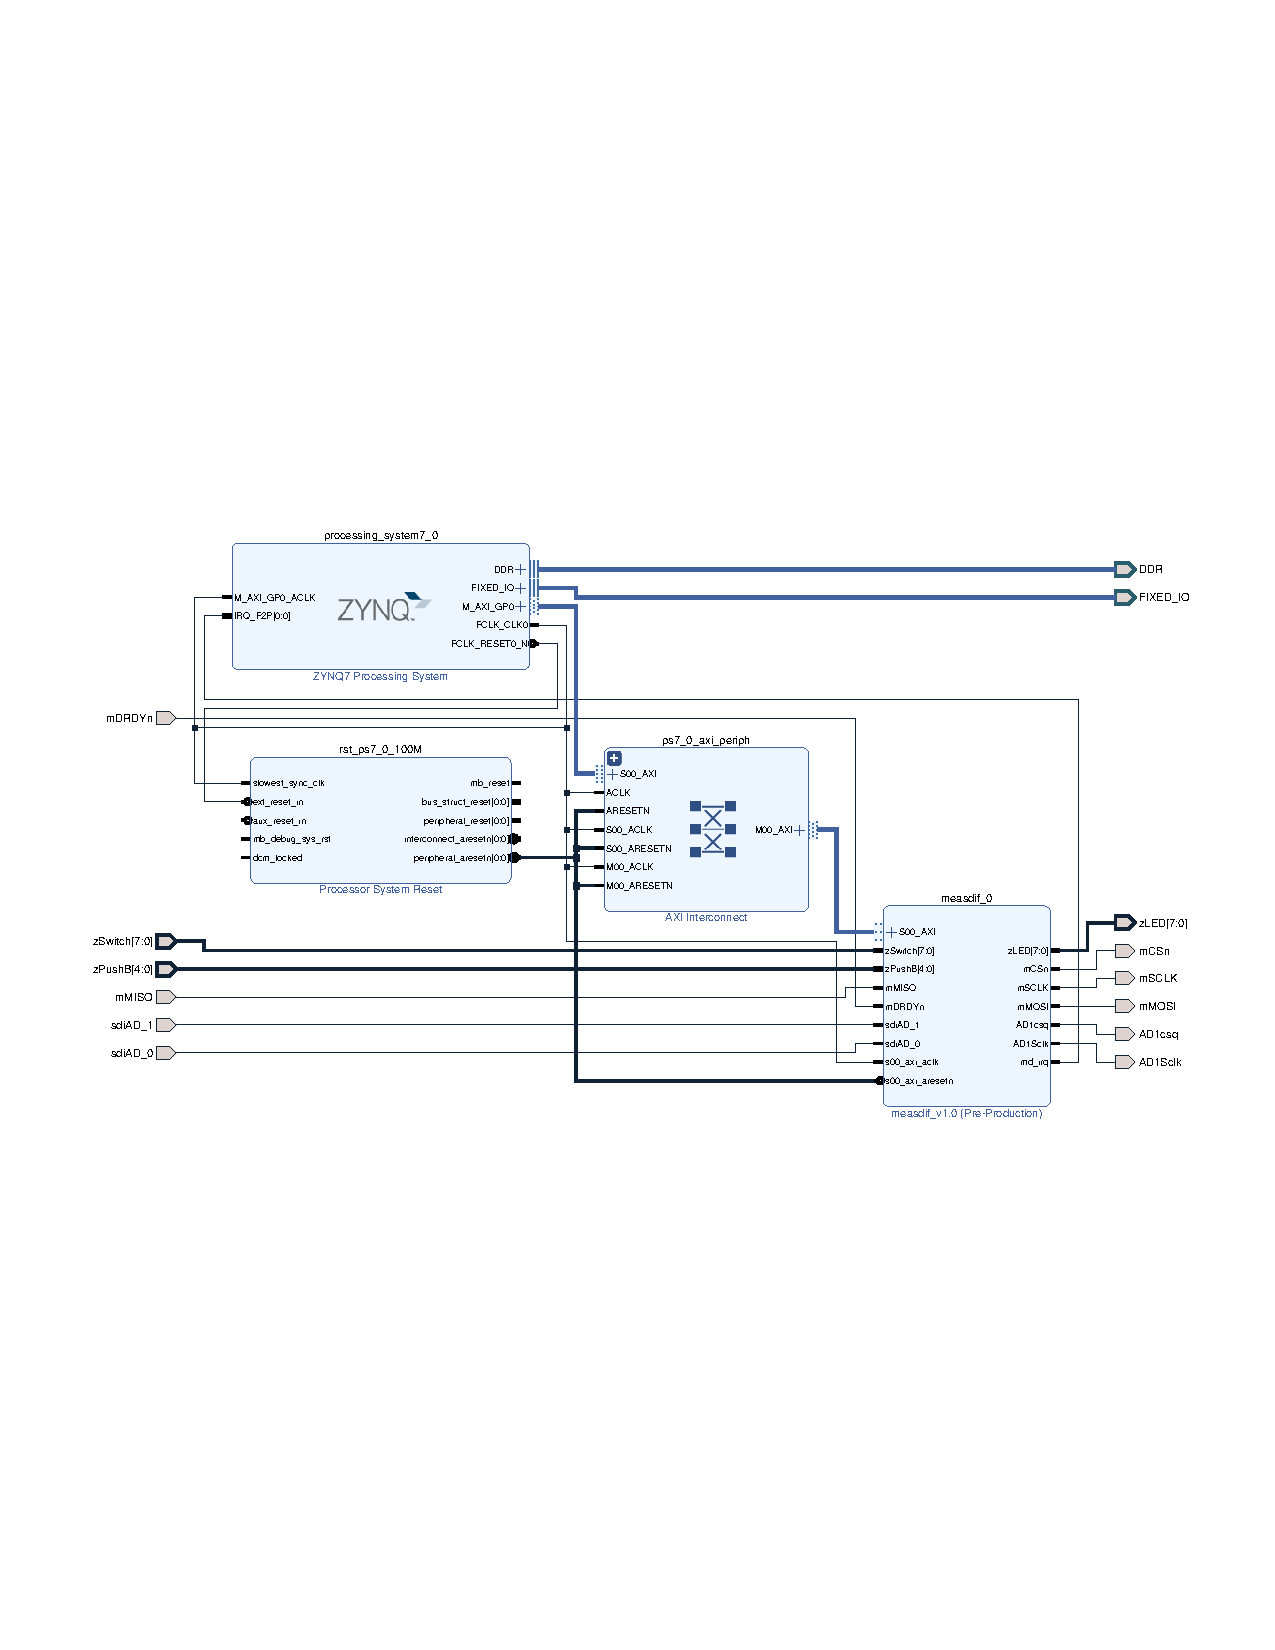
\includegraphics[width = \textwidth, trim = 1.5cm 8cm 1.5cm 8cm, clip]{media/zedbmg_sys.pdf}
\caption{Block Diagram of the whole system in Vivado}
\end{center}
\end{figure} 

After making the block diagram inside Vivado, the design has to be synthesized and for the synthesis first a constraint file for the board has to be written. The constraint file (.xdc file) define the hardware on the board such as Switches and Push Buttons which are used for this project. It specifies which pins to be used for which input and output. Since we are using the Zedboard FPGA developing board we need to write the constraint file for this board. \\
The following code shows the complete contraint file used for this project. 
\begin{minted}[breaklines, tabsize = 4, bgcolor = lightgray, numbers = left]{tcl}
############################
# On-board leds            #
############################
# all 8 leds
set_property PACKAGE_PIN T22 [get_ports zLED[0]]
set_property PACKAGE_PIN T21 [get_ports zLED[1]]
set_property PACKAGE_PIN U22 [get_ports zLED[2]]
set_property PACKAGE_PIN U21 [get_ports zLED[3]]
set_property PACKAGE_PIN V22 [get_ports zLED[4]]
set_property PACKAGE_PIN W22 [get_ports zLED[5]]
set_property PACKAGE_PIN U19 [get_ports zLED[6]]
set_property PACKAGE_PIN U14 [get_ports zLED[7]]
set_property IOSTANDARD LVCMOS33 [get_ports zLED]

# zSwitch [7:0]
############################
# On-board switches        #
############################
set_property PACKAGE_PIN F22 [get_ports zSwitch[0]]
set_property PACKAGE_PIN G22 [get_ports zSwitch[1]]
set_property PACKAGE_PIN H22 [get_ports zSwitch[2]]
set_property PACKAGE_PIN F21 [get_ports zSwitch[3]]
set_property PACKAGE_PIN H19 [get_ports zSwitch[4]]
set_property PACKAGE_PIN H18 [get_ports zSwitch[5]]
set_property PACKAGE_PIN H17 [get_ports zSwitch[6]]
set_property PACKAGE_PIN M15 [get_ports zSwitch[7]]
set_property IOSTANDARD LVCMOS18 [get_ports zSwitch]

# zPushB [4:0]
############################
# On-board pushbuttons     #
############################
set_property PACKAGE_PIN P16 [get_ports zPushB[0]]
set_property PACKAGE_PIN R16 [get_ports zPushB[1]]
set_property PACKAGE_PIN N15 [get_ports zPushB[2]]
set_property PACKAGE_PIN R18 [get_ports zPushB[3]]
set_property PACKAGE_PIN T18 [get_ports zPushB[4]]
set_property IOSTANDARD LVCMOS18 [get_ports zPushB]


# PMOD JA
############################
# PmodAD1                 #
############################
#NET JA1         LOC = Y11   | IOSTANDARD=LVCMOS33;
#NET JA2         LOC = AA11  | IOSTANDARD=LVCMOS33;
#NET JA3         LOC = Y10   | IOSTANDARD=LVCMOS33;
#NET JA4         LOC = AA9   | IOSTANDARD=LVCMOS33;
set_property PACKAGE_PIN Y11 [get_ports AD1csq]
set_property IOSTANDARD LVCMOS33 [get_ports AD1csq]
set_property PACKAGE_PIN AA9 [get_ports AD1Sclk]
set_property IOSTANDARD LVCMOS33 [get_ports AD1Sclk]
set_property PACKAGE_PIN Y10 [get_ports sdiAD_1]
set_property IOSTANDARD LVCMOS33 [get_ports sdiAD_1]
set_property PACKAGE_PIN AA11 [get_ports sdiAD_0]
set_property IOSTANDARD LVCMOS33 [get_ports sdiAD_0]


# PMOD JC1
############################
# MAXPMB1#                 #
############################
#NET JC1_N         LOC = AB6  | IOSTANDARD=LVCMOS33;  # "JC1_N" - 2
#NET JC1_P         LOC = AB7  | IOSTANDARD=LVCMOS33;  # "JC1_P" - 1
#NET JC2_N         LOC = AA4  | IOSTANDARD=LVCMOS33;  # "JC2_N" - 4
#NET JC2_P         LOC = Y4   | IOSTANDARD=LVCMOS33;  # "JC2_P" - 3
#NET JC3_N         LOC = T6   | IOSTANDARD=LVCMOS33;  # "JC3_N" - 8
#NET JC3_P         LOC = R6   | IOSTANDARD=LVCMOS33;  # "JC3_P" - 7
#NET JC4_N         LOC = U4   | IOSTANDARD=LVCMOS33;  # "JC4_N" -10
#NET JC4_P         LOC = T4   | IOSTANDARD=LVCMOS33;  # "JC4_P" - 9
set_property PACKAGE_PIN AB7 [get_ports mCSn]
set_property IOSTANDARD LVCMOS33 [get_ports mCSn]
set_property PACKAGE_PIN AB6 [get_ports mMOSI]
set_property IOSTANDARD LVCMOS33 [get_ports mMOSI]
set_property PACKAGE_PIN Y4 [get_ports mMISO]
set_property IOSTANDARD LVCMOS33 [get_ports mMISO]
set_property PACKAGE_PIN AA4 [get_ports mSCLK]
set_property IOSTANDARD LVCMOS33 [get_ports mSCLK]
set_property PACKAGE_PIN R6 [get_ports mDRDYn]
set_property IOSTANDARD LVCMOS33 [get_ports mDRDYn]

\end{minted}

After adding the constraint file, the design, and HDL wrapper is generated for the whole design, since the block diagram design is not synthesizable. After HDL wrapper is generated the design is synthesized inside Vivado and after synthesization, the bitstream is generated for the design. \\
After generation of the bistream, the generated hardware should be exported in .xsa format to use it for software development either in Bare Metal Programming or Embedded Linux Programming. 
